\documentclass[12pt,a4paper]{report}
\usepackage[utf8]{inputenc}
\usepackage[T1]{fontenc}
\usepackage{mathpazo}
\usepackage[margin=2.5cm]{geometry}
\usepackage{graphicx}
\usepackage{booktabs}
\usepackage{amsmath,amssymb}
\usepackage{hyperref}
\usepackage[numbers]{natbib}
\usepackage{caption}
\usepackage{float}
\usepackage{longtable}
\usepackage{enumitem}
\usepackage{xcolor}
\usepackage{tabularx}
\usepackage{multirow}
\usepackage{tikz}
\usetikzlibrary{positioning,arrows.meta,shapes.geometric,fit}

\usepackage{fancyhdr}
\pagestyle{fancy}
\fancyhf{}
\fancyhead[L]{\leftmark}
\fancyhead[R]{\thepage}
\renewcommand{\headrulewidth}{0.4pt}
\fancypagestyle{plain}{
  \fancyhf{}
  \fancyfoot[C]{\thepage}
  \renewcommand{\headrulewidth}{0pt}
}

\bibliographystyle{unsrt}

\hypersetup{
  colorlinks=true,
  linkcolor=blue!60!black,
  citecolor=blue!60!black,
  urlcolor=blue!60!black
}

\title{\textbf{HYDRA: Explainability-Driven Intrusion Detection\\for IoT Network-Flow Data}}
\author{Varatt Saengsiripongpun\\[1em]
Bachelor of Science (Honours) in\\Computer Science and Artificial Intelligence\\[1em]
The University of Bath\\[1em]
April 2026}
\date{}

\begin{document}
\pagenumbering{roman}

% ============================================================
% TITLE PAGE
% ============================================================
\begin{titlepage}
\centering
\vspace*{\fill}
\vspace*{-2cm}
{\LARGE\bfseries HYDRA: Explainability-Driven Intrusion Detection\\[0.3em] for IoT Network-Flow Data\par}
\vspace{2cm}
{\Large Varatt Saengsiripongpun\par}
\vspace{1.5cm}
{\large Bachelor of Science (Honours) in\\Computer Science and Artificial Intelligence\par}
\vspace{1cm}
{\large The University of Bath\par}
\vspace{0.5cm}
{\large April 2026\par}
\vspace*{\fill}
\vspace*{\fill}
\end{titlepage}

% ============================================================
% COPYRIGHT
% ============================================================
\newpage
\thispagestyle{empty}
\section*{Copyright}
Attention is drawn to the fact that copyright of this dissertation rests with its author. The Intellectual Property Rights of the products produced as part of the project belong to the author unless otherwise specified below, in accordance with the University of Bath's policy on intellectual property (see \url{https://www.bath.ac.uk/publications/university-ordinances/}).

This copy of the dissertation has been supplied on condition that anyone who consults it is understood to recognise that its copyright rests with its author and that no quotation from the dissertation and no information derived from it may be published without the prior written consent of the author.

\section*{Declaration}
This dissertation is submitted to the University of Bath in accordance with the requirements of the degree of Bachelor of Science in the Department of Computer Science. No portion of the work in this dissertation has been submitted in support of an application for any other degree or qualification of this or any other university or institution of learning. Except where specifically acknowledged, it is the work of the author.

% ============================================================
% ABSTRACT
% ============================================================
\newpage
\begin{abstract}
Machine-learning-based Intrusion Detection Systems (IDS) achieve high benchmark performance yet frequently operate as opaque black boxes, issuing alerts without reliable justification. This opacity creates direct operational costs: analysts must investigate alerts without trustworthy guidance, false positives generate alert fatigue, and trust in automated detection degrades even when headline accuracy is strong.

This dissertation presents HYDRA, an explainability-driven IDS framework that treats model explanations as measurable system outputs. HYDRA addresses two tasks simultaneously: binary attack detection and multi-class attack-type classification, reflecting the operational need to know both that an anomaly has occurred and which threat category it represents. The core model set comprises majority-class and threshold baselines, Logistic Regression (as a reference explainer), Random Forest, XGBoost, and LightGBM, evaluated on TON\_IoT as the primary benchmark and CIC-IoT-2023 for generalisation. A CNN-LSTM model achieves PR-AUC of 0.9998 on TON\_IoT; a Graph Neural Network achieves PR-AUC of 0.9997.

Explanations are generated using a portfolio of post-hoc methods matched to each model family: SHAP TreeExplainer for the tree ensembles, SHAP LinearExplainer for Logistic Regression, and LIME applied model-agnostically across all models. Integrated Gradients is implemented for the CNN-LSTM and GNN extensions. Every explanation method is evaluated against five measurable criteria: faithfulness (comprehensiveness and sufficiency under top-$k$ feature ablation), stability (Spearman rank correlation under noise perturbation and across independent retraining runs), simplicity ($k_{90}$ fraction and Gini coefficient), plausibility (RMA@$k$ against expert network features), and timeliness (milliseconds per sample).

The contribution is not a novel detection algorithm but a reproducible evaluation framework that operationalises explainability as a measurable system property, enabling rigorous assessment of whether high-performing IDS models can provide explanations that are faithful, stable, and useful enough to support analyst decision-making in practice.

On TON\_IoT, all four tabular models achieve PR-AUC of 1.000 and ROC-AUC of 1.000 under the behaviour-only regime, with XGBoost achieving the highest OXS explanation quality score of 0.828. Cross-dataset evaluation on CIC-IoT-2023 reveals that tree ensemble models suffer catastrophic ROC-AUC drops of up to 87\%, while Logistic Regression generalises most robustly (ROC-AUC drop of 7.3\%). The leakage interaction analysis demonstrates that including identifier features reduces explanation plausibility by 35 percentage points (Cohen's $d = -2.985$) without affecting detection performance.
\end{abstract}

% ============================================================
% TABLE OF CONTENTS
% ============================================================
\tableofcontents
\listoftables
\listoffigures

\chapter*{Glossary of Abbreviations}
\addcontentsline{toc}{chapter}{Glossary of Abbreviations}

\begin{longtable}{p{3cm}p{10cm}}
\textbf{Abbreviation} & \textbf{Definition} \\
\midrule
AOPC & Area Over the Perturbation Curve \\
AUC & Area Under the Curve \\
CNN & Convolutional Neural Network \\
DoS & Denial of Service \\
GNN & Graph Neural Network \\
IDS & Intrusion Detection System \\
IG & Integrated Gradients \\
IoT & Internet of Things \\
LIME & Local Interpretable Model-agnostic Explanations \\
LSTM & Long Short-Term Memory \\
OXS & Operational eXplainability Score \\
PR-AUC & Precision-Recall Area Under the Curve \\
RF & Random Forest \\
ROC-AUC & Receiver Operating Characteristic AUC \\
SHAP & SHapley Additive exPlanations \\
SOC & Security Operations Centre \\
XAI & Explainable Artificial Intelligence \\
\end{longtable}

% ============================================================
% CHAPTER 1: INTRODUCTION
% ============================================================
\pagenumbering{arabic}
\pagestyle{fancy}
\chapter{Introduction}
\label{ch:introduction}

\section{Motivation}
\label{sec:motivation}

The cyber-defence landscape is defined by a fundamental asymmetry: defenders must secure an ever-expanding and heterogeneous attack surface, while adversaries require only a single successful compromise. Automated scanning and exploitation infrastructure operates at tens of thousands of scans per second, and credential-based attacks have risen markedly \cite{fortinet2025}. Simultaneously, enterprises generate billions of telemetry events per day across servers, endpoints, cloud services, and IoT devices, creating a signal-to-noise problem that overwhelms traditional monitoring and human analysts \cite{dang2019}.

Conventional controls---signature-based IDS (Snort, Suricata) and rule-driven SIEM platforms---are fundamentally reactive: they cannot detect novel attacks, polymorphic malware, or living-off-the-land techniques \cite{ahmad2021}, and produce high false positive rates as system complexity grows \cite{zhu2023}.

AIOps for cybersecurity seeks to address these limitations by embedding machine learning into the Security Operations Centre (SOC). Industry analyses suggest alert noise reductions of 70--90\% \cite{dang2023,nguyen2024}. However, learned models introduce new operational challenges: deep learning systems behave as opaque black boxes, real-time inference imposes strict latency constraints, and models are vulnerable to concept drift and adversarial manipulation \cite{schwarzschild2021,goldblum2023}.

\section{Problem Statement}
\label{sec:problem}

A central failing of current IDS research is the gap between detection performance and operational usefulness. High benchmark accuracy on public datasets does not translate directly into deployable, trustworthy systems for three interconnected reasons.

First, many published results are inflated by evaluation leakage. When network-flow records are split randomly by row, similar traffic from the same hosts appears in both training and test sets, allowing models to recognise identity patterns rather than attack behaviour \cite{turcotte2018}. This leakage is invisible under standard evaluation but causes catastrophic degradation in deployment.

Second, most IDS models provide binary outputs without indicating the threat category. In practice, different attack types---denial-of-service, ransomware, exfiltration, scanning---require different analyst responses. Dual-task detection and classification is substantially more useful operationally.

Third, accurate models are underutilised because alerts lack justification. When a model flags a flow as malicious without explaining which features triggered the decision, analysts must investigate blindly, increasing triage time and eroding trust in automation.

\section{Aim and Objectives}
\label{sec:aim}

The aim of this project is to design, implement, and evaluate HYDRA: an intrusion detection framework that addresses both binary attack detection and multi-class attack-type classification, while generating per-alert explanations that are systematically validated for reliability, consistency, and operational usefulness on IoT network-flow data.

The specific objectives are:
\begin{enumerate}
  \item To implement and evaluate a structured model progression---from baselines through tabular ensemble models and deep learning architectures---for both binary and multi-class intrusion detection on TON\_IoT, with CIC-IoT-2023 as a secondary generalisation benchmark. A CNN-LSTM model and a Graph Neural Network (GraphSAGE with Integrated Gradients attribution) are evaluated as deep learning extensions.
  \item To define and apply two feature regimes that explicitly isolate and quantify the contribution of identifier leakage to detection performance and explanation quality.
  \item To generate standardised per-alert explanation records for tabular models using SHAP TreeExplainer, for the Logistic Regression reference model using SHAP LinearExplainer, and for all models using LIME as a model-agnostic cross-reference. Integrated Gradients is implemented for the CNN-LSTM and GNN extensions.
  \item To evaluate explanations systematically using five measurable criteria: faithfulness (comprehensiveness and sufficiency), stability (under noise perturbation and across independent retraining seeds), simplicity ($k_{90}$ and Gini), plausibility (RMA@$k$), and timeliness (ms per sample).
  \item To position HYDRA explicitly against concurrent XAI-IDS work and compare the performance--explainability trade-off across model types, with generalisation evaluation on CIC-IoT-2023 where feasible.
\end{enumerate}

\section{Research Questions}
\label{sec:rqs}

This project is structured around four research questions:

\noindent\textbf{RQ1 (Detection):} Which modelling approach provides the strongest performance for both binary attack detection and multi-class attack-type classification on tabular network-flow features, when evaluated using operationally relevant metrics such as PR-AUC and false positive rate at a fixed recall target?

\noindent\textbf{RQ2 (Explainability):} To what extent can the best-performing detector provide per-alert, feature-level explanations with high and consistent coverage across both detection tasks?

\noindent\textbf{RQ3 (Reliability):} How stable are explanation outputs across repeated training runs and different data conditions, and does stability differ between the binary and multi-class tasks?

\noindent\textbf{RQ4 (Faithfulness):} Do model-generated explanations exhibit fidelity---that is, does removing the highlighted features significantly change model confidence---and do explanation patterns align with known network intrusion behaviours for each attack type?

\section{Contributions}
\label{sec:contributions}

This project does not propose a novel detection algorithm. Its contributions are:
\begin{itemize}
  \item A reproducible IDS pipeline that supports both binary and multi-class intrusion detection with standardised per-alert explanation records for tabular ensembles, with CNN-LSTM (PR-AUC $= 0.9998$) and GNN (PR-AUC $= 0.9997$) deep learning extensions producing valid detection results and Integrated Gradients attributions.
  \item A unified, implementation-ready explainability evaluation protocol covering five measurable criteria (faithfulness, stability, simplicity, plausibility, timeliness), applied consistently across all evaluated model families and both detection tasks. Importantly, the stability criterion is operationalised as two separate experiments: seed-retraining stability (training $S = 5$ models with different random seeds) and noise-perturbation robustness (perturbing fixed model inputs), which address distinct aspects of explanation reliability.
  \item Empirical analysis of the impact of identifier-based feature leakage on detection performance and explanation quality in IoT network-flow datasets, and explicit positioning of HYDRA against concurrent XAI-IDS systems through a gap analysis table.
  \item A systematic empirical analysis of how evaluation methodology---specifically the choice of data splitting strategy---inflates both detection and classification performance in IoT intrusion detection. Host-disjoint evaluation reduces the best model's multiclass macro-F1 from 1.000 to 0.742 (Random Forest) and XGBoost's binary ROC-AUC from 1.000 to 0.842, even when identifier features are excluded, demonstrating that host-level flow correlation is a previously underreported source of evaluation leakage.
\end{itemize}

To the best of the author's knowledge, HYDRA is the first system to empirically implement and validate all of the following simultaneously: (i) dual-task binary and multiclass detection evaluated under leakage-controlled feature regimes, (ii) a five-criterion quantitative XAI evaluation protocol producing a composite OXS score, (iii) cross-dataset generalisation testing on IoT-specific benchmarks, and (iv) empirical measurement of the interaction between identifier leakage and explanation quality. While individual components appear in the literature (Table~\ref{tab:positioning}), their combined application to IoT intrusion detection with measurable explanation evaluation is novel.

\begin{table}[H]
\caption{Summary of HYDRA's contributions and their relation to research gaps.}
\label{tab:contributions}
\centering
\begin{tabular}{p{0.28\textwidth}p{0.35\textwidth}p{0.28\textwidth}}
\toprule
\textbf{Contribution} & \textbf{Gap Addressed} & \textbf{Key Evidence} \\
\midrule
Dual-task IDS pipeline & Binary-only detection (\S\ref{sec:binary-only}) & Macro-F1 = 1.000 (Ch.~\ref{ch:results}) \\
Five-criterion XAI protocol & XAI as afterthought (\S\ref{sec:xai-afterthought}) & OXS ranking (Table~\ref{tab:oxs}) \\
Leakage interaction analysis & Evaluation leakage (\S\ref{sec:leakage-gap}) & RMA@5 $\Delta$ = -0.35 (Table~\ref{tab:leakage}) \\
Cross-dataset generalisation & Single-dataset evaluation & ROC-AUC drop up to 87\% (Table~\ref{tab:cross}) \\
Split-strategy leakage analysis & Overoptimistic benchmarks & Macro-F1: 1.000 $\to$ 0.742 (Table~\ref{tab:host-multiclass}) \\
\bottomrule
\end{tabular}
\end{table}

\section{Dissertation Structure}
\label{sec:structure}

Chapter~\ref{ch:literature} presents the literature, technology, and data survey. Chapter~\ref{ch:methodology} describes the HYDRA methodology. Chapter~\ref{ch:results} presents experimental results. Chapter~\ref{ch:discussion} discusses findings, trade-offs, and limitations. Chapter~\ref{ch:conclusions} concludes and identifies future work.

% ============================================================
% CHAPTER 2: LITERATURE REVIEW
% ============================================================
\chapter{Literature, Technology and Data Survey}
\label{ch:literature}

\section{Evolution of Intrusion Detection}
\label{sec:evolution}

Intrusion detection has evolved through three generations. Signature-based systems (Snort, Suricata) match packet contents against known Indicators of Compromise, offering high precision for catalogued threats but fundamentally unable to detect novel attacks, polymorphic variants, or adversaries using legitimate credentials \cite{ahmad2021}. Rule-based SIEM platforms extend this by correlating events across sources, but static rules become brittle as system complexity grows and produce high false positive rates on heterogeneous telemetry \cite{zhu2023}.

Anomaly-based IDS addressed the zero-day gap by learning statistical baselines of normal behaviour. Supervised ML methods---Random Forest, SVMs, gradient boosting---achieved high accuracy on benchmarks such as KDD Cup 99 and CICIDS2017 \cite{aldweesh2020}, though they generalise poorly to unseen attack types and suffer concept drift. Hybrid architectures combining supervised classification with unsupervised anomaly detection improve zero-day recall \cite{alsaedi2020}, a principle that underpins HYDRA's design.

AIOps platforms automate IT security operations through ML-driven noise reduction, correlation, and root-cause analysis \cite{dang2019}. Industry analyses suggest alert noise reductions of 70--90\% \cite{dang2023,fortinet2025}, though commercial platforms are closed and not benchmarked on standardised open datasets. HYDRA provides a transparent, reproducible alternative.

\section{Supervised and Unsupervised Learning for Cyber Defence}
\label{sec:supervised}

\subsection{Supervised Ensemble Methods}
\label{sec:ensemble}

Ensemble tree methods form the core of HYDRA's tabular detection pipeline. Random Forest \cite{breiman2001} constructs an ensemble of independently trained decision trees via bootstrap sampling with random feature subsets, producing stable feature importance estimates. XGBoost \cite{chen2016} implements gradient boosted trees through second-order gradient approximation and regularisation. LightGBM \cite{ke2017} extends this through histogram-based splitting for memory efficiency. Logistic Regression serves as a reference explainer whose linear decision boundary yields deterministic, auditable attributions.

In the IDS literature, ensemble models consistently achieve state-of-the-art results \cite{shtayat2023,rani2024}, though many studies use random row-level splits without temporal ordering, raising concerns about evaluation leakage. A key challenge for supervised IDS is class imbalance: standard accuracy metrics are misleading when attack events represent a small fraction of total traffic, making precision-recall metrics and PR-AUC essential for operational evaluation.

\subsection{Unsupervised Methods}
\label{sec:unsupervised}

Isolation Forest \cite{liu2008} isolates anomalies by recursively partitioning the feature space with random cuts; anomalous points require fewer partitions. It operates in approximately linear time, making it practical as a fast pre-filter \cite{alsaedi2020}. Autoencoders trained on normal traffic detect anomalies via high reconstruction error \cite{moustafa2021}; LSTM-autoencoders extend this to sequential data \cite{malhotra2016,park2023}. HYDRA does not use these methods directly but they inform its design philosophy.

\section{Deep Learning for Log and Network-Flow Analysis}
\label{sec:deeplearning}

DeepLog \cite{du2017} treats log entries as sequences of discrete keys and trains an LSTM to predict the next expected key, flagging deviations as anomalies. LogBERT \cite{guo2021} adapts BERT's masked prediction to log sequences, conditioning on both left and right context for improved detection. Transformer-based models achieve higher accuracy than LSTM baselines on LogHub benchmarks but at substantially higher computational cost \cite{guo2021,le2023}.

For network flow data, hybrid CNN-LSTM architectures capture both spatial (feature interaction) and temporal (sequence) structure simultaneously. Studies on TON\_IoT demonstrate detection accuracy above 99\% for binary classification \cite{ferrag2022,imrana2021}. Federated variants \cite{popoola2021} keep raw traffic local to each device, addressing privacy constraints in distributed IoT environments.

\section{Graph-Based Detection and Predictive Analytics}
\label{sec:graphbased}

Network communications have natural graph structure: hosts are nodes and flows are edges. GNNs exploit this relational structure through message-passing operations, learning representations that capture communication topology---particularly relevant for detecting scanning, lateral movement, and botnet coordination. Euler \cite{king2023} uses temporal link prediction and LMTracker \cite{fangY2022} employs heterogeneous graph embedding for lateral movement detection on authentication graphs.

Predictive analytics extends detection to forecasting. LSTM-based approaches forecast DDoS intensity \cite{kong2025}, and sequence models on authentication patterns predict lateral movement by flagging low-probability authentications \cite{turcotte2018}. A survey of data-driven methods \cite{chou2021} identifies evaluation metrics, dataset selection, and reliability under concept drift as primary challenges.

\section{Explainability in Intrusion Detection}
\label{sec:xai}

\subsection{The Explainability Problem in IDS}
\label{sec:xai-problem}

High-performing ML models used for intrusion detection frequently operate as black boxes, producing alerts without exposing the features or reasoning behind them. This increases triage time, compounds alert fatigue, and erodes the trust required for automation in high-stakes SOC environments. Post-hoc XAI methods explain already-trained models without modifying them, and are more widely used than intrinsically interpretable models because they can be applied to high-performing ensembles \cite{adadi2018}.

HYDRA implements four complementary post-hoc methods: SHAP TreeExplainer for tree ensembles, SHAP LinearExplainer for Logistic Regression, LIME as a model-agnostic cross-reference, and Integrated Gradients for the CNN-LSTM and GNN.

\subsection{SHAP TreeExplainer}
\label{sec:shap-tree}

SHAP \cite{lundberg2017} grounds feature attribution in cooperative game theory, computing each feature's Shapley value---its average marginal contribution across all possible feature orderings. TreeExplainer \cite{lundberg2020} provides an exact, polynomial-time implementation for tree-based models, avoiding the sampling approximation of model-agnostic variants. In HYDRA, TreeExplainer produces both local per-alert attributions and global feature importance rankings. SHAP values can be unstable under correlated features, which HYDRA addresses through explicit stability measurement.

\subsection{SHAP LinearExplainer}
\label{sec:shap-linear}

For Logistic Regression, LinearExplainer computes Shapley values analytically by exploiting the additive structure of linear prediction. Because attributions are deterministic given the same data, LogReg serves as a stability anchor for comparing against tree ensemble models, consistent with the performance--explainability trade-off analysis of \cite{bhatt2020} and \cite{adadi2018}.

\subsection{LIME}
\label{sec:lime}

LIME \cite{ribeiro2016} explains individual predictions by fitting a locally linear surrogate model to perturbed versions of the input. HYDRA applies LIME across all models as a model-agnostic cross-reference against SHAP attributions. LIME's primary limitation is sampling variance; comparative studies find SHAP more stable for tabular data \cite{kalakoti2025}, so HYDRA treats LIME as a secondary method.

\subsection{Integrated Gradients}
\label{sec:ig}

Integrated Gradients \cite{sundararajan2017} computes feature attributions by integrating the model's gradients along a path from a baseline input to the actual input. It satisfies sensitivity and implementation invariance axioms. In HYDRA, IG is applied to both the CNN-LSTM and the GNN's edge feature space.

\subsection{GNNExplainer and Policy Graphs}
\label{sec:gnnexplainer}

GNNExplainer \cite{ying2019} learns a soft mask over a node's computational subgraph that maximises mutual information with the full-graph prediction. Subgraph explanations can be non-unique and may be dominated by topology rather than feature content. Policy graphs \cite{alves2017} and provenance graphs \cite{fang2022} represent access control and causal event chains, informing the plausibility criterion in HYDRA's evaluation.

\subsection{XAI Evaluation: Five Criteria}
\label{sec:xai-eval}

A recurring weakness in XAI-IDS research is the absence of systematic evaluation of explanations. HYDRA evaluates every method against five criteria (Table~\ref{tab:five-criteria}).

\begin{table}[H]
\centering
\caption{HYDRA's five-criterion XAI evaluation framework.}
\label{tab:five-criteria}
\small
\begin{tabularx}{\textwidth}{lp{3.5cm}X}
\toprule
\textbf{Criterion} & \textbf{Metric} & \textbf{Description} \\
\midrule
Faithfulness & Comprehensiveness + Sufficiency (top-$k$ ablation) & Remove top-$k$ features (comprehensiveness) or keep only top-$k$ (sufficiency) and measure confidence change. \\
\addlinespace
Stability & S1: Spearman $\rho$ across $S = 5$ retraining runs; S2: Spearman $\rho$ under Gaussian noise & Two distinct experiments addressing training stochasticity (RQ3) and input perturbation (RQ4). \\
\addlinespace
Simplicity & $k_{90}$ fraction + Gini coefficient & Minimum features for 90\% attribution mass (normalised); concentration of attribution distribution. \\
\addlinespace
Plausibility & RMA@$k$ vs expert features & Proportion of top-$k$ attributed features in an expert-defined reference set. \\
\addlinespace
Timeliness & ms per sample & Wall-clock time for a complete explanation record. \\
\bottomrule
\end{tabularx}
\end{table}

Faithfulness is measured through top-$k$ ablation: comprehensiveness removes the top-$k$ features and measures confidence drop; sufficiency retains only top-$k$ and measures whether they reproduce the original confidence \cite{bhatt2020,deyoung2020}. Stability uses Spearman rank correlation, which captures the full ordering of feature importance and is robust to ties. Simplicity combines $k_{90}$ (fraction of features needed for 90\% of attribution mass) with the Gini coefficient of the attribution distribution. Plausibility compares top-$k$ features against expert-defined reference sets for each attack type. Timeliness constrains which methods are viable for real-time deployment.

\section{Positioning HYDRA Against Concurrent Work}
\label{sec:positioning}

Four recent papers address XAI-IDS in settings sufficiently similar to HYDRA that explicit positioning is necessary. Table~\ref{tab:positioning} maps each against HYDRA's principal design choices.

\begin{table}[H]
\centering
\caption{Positioning HYDRA against concurrent XAI-IDS work. \checkmark = present, $\circ$ = partial, $\times$ = absent.}
\label{tab:positioning}
\small
\begin{tabular}{lccccc}
\toprule
\textbf{Dimension} & \textbf{HYDRA} & \textbf{E-XAI} & \textbf{XAI-IDS} & \textbf{Frontiers} & \textbf{TalTech} \\
 & & \cite{arreche2024} & \cite{arreche2024b} & \cite{mohale2025} & \cite{kalakoti2025} \\
\midrule
Binary + multi-class detection & \checkmark & $\times$ & $\times$ & $\times$ & $\times$ \\
Leakage-controlled feature regimes & \checkmark & $\times$ & $\times$ & $\times$ & $\times$ \\
Temporal (non-random) splitting & \checkmark & $\times$ & $\times$ & $\circ$ & $\times$ \\
$\geq$3 XAI methods compared & \checkmark & \checkmark & \checkmark & $\circ$ & \checkmark \\
Stability measured quantitatively & \checkmark & $\times$ & $\times$ & $\times$ & $\circ$ \\
Timeliness (ms/sample) measured & \checkmark & $\times$ & $\times$ & $\times$ & $\times$ \\
Simplicity ($k_{90}$, Gini) measured & \checkmark & $\times$ & $\times$ & $\times$ & $\times$ \\
Plausibility (RMA@$k$) measured & \checkmark & $\times$ & $\times$ & $\times$ & $\times$ \\
IoT-specific dataset (TON\_IoT) & \checkmark & $\times$ & $\circ$ & \checkmark & $\times$ \\
Cross-dataset generalisation & \checkmark & $\times$ & $\times$ & $\times$ & $\times$ \\
\bottomrule
\end{tabular}
\end{table}

E-XAI \cite{arreche2024} evaluates SHAP, LIME, and IG on deep-learning NIDS but addresses binary classification only, without leakage-controlled features, quantitative stability, or cross-dataset generalisation. XAI-IDS \cite{arreche2024b} applies SHAP and LIME to CICIDS2017 with random splitting and no quantitative XAI evaluation. The Frontiers study \cite{mohale2025} applies SHAP, LIME, and ELI5 but is primarily qualitative. The TalTech study \cite{kalakoti2025} compares four XAI methods on real SOC data using a four-criterion framework, finding DeepLIFT superior to SHAP; HYDRA's addition of timeliness and simplicity criteria, IoT-specific focus, and multi-class evaluation are key differentiators.

Two further works warrant acknowledgement. \cite{adadi2018} propose a conceptual framework for the tension between detection, efficiency, and explanation quality, but without empirical implementation. \cite{sengupta2026} introduce a domain-agnostic explanation reliability index but do not address IDS-specific evaluation. HYDRA is the first system to implement and validate all ten dimensions simultaneously.

\section{Gaps in Current Technology}
\label{sec:gaps}

\subsection{Evaluation Leakage and Overoptimistic Benchmarks}
\label{sec:leakage-gap}

A pervasive problem in IDS research is evaluation leakage that inflates performance. Random row-level splitting places correlated flows from the same hosts or time windows into both training and test sets, allowing models to recognise identity patterns rather than attack behaviours \cite{lanvin2022}. Including identifier features (IPs, ports, URIs) allows models to memorise which sources were associated with attacks \cite{tareq2022}. HYDRA addresses both through deployment-realistic splits and explicit feature regime comparison.

\subsection{Binary-Only Detection}
\label{sec:binary-only}

Most published IDS models evaluate solely binary classification despite operational response differing substantially by threat type. HYDRA's dual-task design addresses this directly.

\subsection{Explainability as a Qualitative Afterthought}
\label{sec:xai-afterthought}

Even IDS studies incorporating explainability present explanations as static plots without measuring stability, fidelity, or coverage. HYDRA's five-criterion framework addresses this gap.

\subsection{Adversarial Robustness and Concept Drift}
\label{sec:adversarial}

Security ML models operate in adversarial environments where attackers may attempt evasion or data poisoning \cite{schwarzschild2021,goldblum2023}, and concept drift renders models obsolete without retraining \cite{gama2014}. HYDRA's modular architecture supports periodic re-evaluation and is designed for extension with drift detection.

\section{Technology Survey}
\label{sec:techsurvey}

HYDRA uses scikit-learn \cite{pedregosa2011} for classical ML and preprocessing, XGBoost and LightGBM for gradient-boosted trees, PyTorch \cite{paszke2019} with PyTorch Geometric \cite{fey2019} for the GNN, SHAP \cite{lundberg2023} for Shapley values, LIME for local surrogate explanations, and Captum for neural network attribution. Apache Kafka \cite{kafka2024} provides streaming infrastructure \cite{raptis2023,martin2022}; Grafana \cite{grafana2023} and Streamlit \cite{streamlit2023} provide visualisation and interactive analyst workbench capabilities.

\section{Data Survey}
\label{sec:datasurvey}

\subsection{TON\_IoT (Primary Dataset)}
\label{sec:toniot}

The TON\_IoT dataset \cite{moustafa2021}, from UNSW Canberra, contains millions of labelled flow records from a realistic IoT testbed spanning nine attack categories: Scanning, DoS, DDoS, Injection, Backdoor, XSS, Ransomware, Password, and MitM. Each record contains binary and categorical labels supporting dual-task evaluation. Known challenges include class imbalance, synthetic attack artefacts, and label leakage through identifier features \cite{ogunseyi2026,ferrag2022}.

\subsection{CIC-IoT-2023 (Generalisation Dataset)}
\label{sec:ciciot}

CIC-IoT-2023 \cite{cic2023} contains approximately 3.18 million flow records after deduplication (44\% duplicates removed), with 34 attack types and 97.7\% attack prevalence. It lacks source IP and timestamp columns, constraining splitting strategies and precluding GNN evaluation. Its greater attack diversity makes it a useful generalisation testbed.

\subsection{Supporting Datasets}
\label{sec:supporting-data}

LogHub \cite{zhu2023} aggregates labelled log datasets (HDFS, BGL, Thunderbird) used as benchmarks for log anomaly detection methods. The LANL dataset \cite{turcotte2018} contains billions of de-identified authentication events from an enterprise network with embedded Red Team activities, informing HYDRA's graph construction approach.

\subsection{Data Preparation}
\label{sec:data-prep}

HYDRA applies consistent preprocessing: feature extraction derives numerical features and protocol flags, class imbalance is addressed through stratified sampling and class-weighted loss functions \cite{anbiaee2025}, temporal splitting respects time-ordering where timestamps are available, and all preprocessing is fitted exclusively on training data.

\section{Summary}
\label{sec:lit-summary}

The literature establishes three conclusions motivating HYDRA. First, ensemble tree methods dominate tabular IDS benchmarks, yet results are frequently inflated by identifier leakage and random splitting, motivating HYDRA's dual-regime evaluation. Second, SHAP provides more stable attributions than LIME for tree models, but LIME's model-agnostic nature makes it the only viable cross-reference across model families, motivating HYDRA's multi-method portfolio. Third, no existing study applies a unified quantitative XAI evaluation protocol across multiple model families on both binary and multi-class IoT detection under leakage-controlled conditions---the primary gap HYDRA addresses.

% ============================================================
% CHAPTER 3: METHODOLOGY
% ============================================================
\chapter{Methodology}
\label{ch:methodology}

\section{Overview}
\label{sec:meth-overview}

HYDRA implements a two-stage classification pipeline: Stage~1 performs binary detection (attack vs.\ normal); Stage~2 classifies detected attacks by type. The experimental design spans three dimensions: \textbf{detection performance} across five ML models and two deep learning architectures under two feature regimes; \textbf{explanation quality} assessed via a five-criterion protocol; and \textbf{cross-dataset generalisation} testing portability of learned representations.

All experiments use TON\_IoT and CIC-IoT-2023. Figure~\ref{fig:pipeline} illustrates the pipeline architecture.

\begin{figure}[H]
\centering
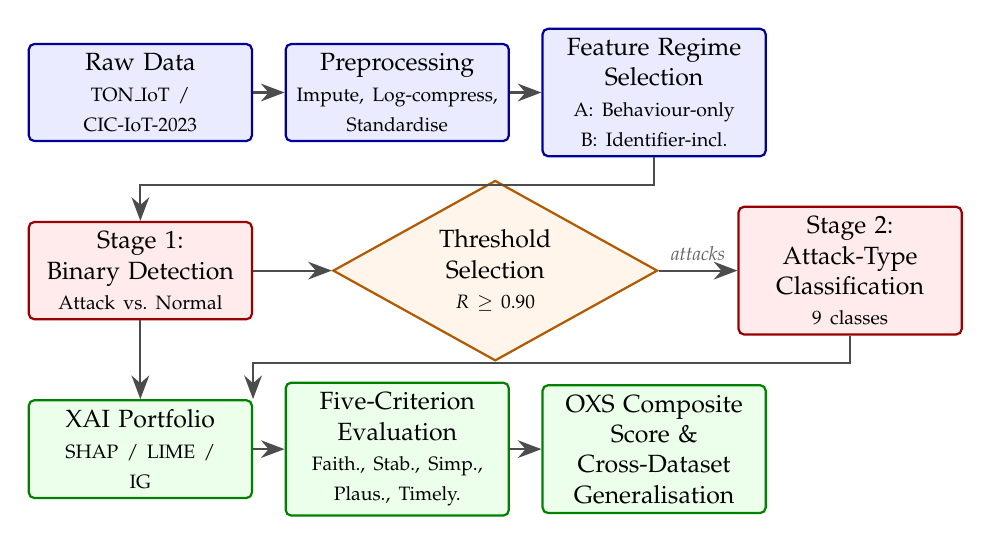
\begin{tikzpicture}[
    node distance=0.6cm and 0.4cm,
    >={Stealth[length=3mm]},
    block/.style={rectangle, draw=blue!60!black, fill=blue!8, text width=2.6cm, minimum height=1.0cm, align=center, font=\small, rounded corners=2pt, line width=0.8pt},
    stage/.style={rectangle, draw=red!60!black, fill=red!8, text width=2.6cm, minimum height=1.0cm, align=center, font=\small, rounded corners=2pt, line width=0.8pt},
    decision/.style={diamond, draw=orange!70!black, fill=orange!8, text width=1.6cm, minimum height=0.8cm, align=center, font=\small, aspect=1.8, line width=0.8pt},
    output/.style={rectangle, draw=green!50!black, fill=green!8, text width=2.6cm, minimum height=1.0cm, align=center, font=\small, rounded corners=2pt, line width=0.8pt},
    arrow/.style={->, line width=0.8pt, draw=black!70},
    label/.style={font=\scriptsize\itshape, text=black!60}
]

% Row 1: Data pipeline
\node[block] (raw) {Raw Data\\{\scriptsize TON\_IoT /}\\{\scriptsize CIC-IoT-2023}};
\node[block, right=of raw] (preproc) {Preprocessing\\{\scriptsize Impute, Log-compress,}\\{\scriptsize Standardise}};
\node[block, right=of preproc] (regime) {Feature Regime\\Selection\\{\scriptsize A: Behaviour-only}\\{\scriptsize B: Identifier-incl.}};

% Row 2: Detection pipeline
\node[stage, below=1.0cm of raw] (stage1) {Stage~1:\\Binary Detection\\{\scriptsize Attack vs.\ Normal}};
\node[decision, right=1.0cm of stage1] (thresh) {Threshold\\Selection\\{\scriptsize $R \geq 0.90$}};
\node[stage, right=1.0cm of thresh] (stage2) {Stage~2:\\Attack-Type\\Classification\\{\scriptsize 9 classes}};

% Row 3: Explanation and evaluation
\node[output, below=1.0cm of stage1] (xai) {XAI Portfolio\\{\scriptsize SHAP / LIME /}\\{\scriptsize IG}};
\node[output, right=of xai] (eval) {Five-Criterion\\Evaluation\\{\scriptsize Faith., Stab., Simp.,}\\{\scriptsize Plaus., Timely.}};
\node[output, right=of eval] (oxs) {OXS Composite\\Score \&\\Cross-Dataset\\Generalisation};

% Arrows Row 1
\draw[arrow] (raw) -- (preproc);
\draw[arrow] (preproc) -- (regime);

% Arrow from Row 1 to Row 2
\draw[arrow] (regime.south) -- ++(0,-0.35) -| (stage1.north);

% Arrows Row 2
\draw[arrow] (stage1) -- (thresh);
\draw[arrow] (thresh) -- node[above, label] {attacks} (stage2);

% Arrows Row 2 to Row 3
\draw[arrow] (stage1.south) -- (xai.north);
\draw[arrow] (stage2.south) -- ++(0,-0.35) -| (xai.north east);

% Arrows Row 3
\draw[arrow] (xai) -- (eval);
\draw[arrow] (eval) -- (oxs);

\end{tikzpicture}
\caption{HYDRA pipeline architecture. Raw data flows through preprocessing and feature regime selection into the two-stage detection pipeline. Both stages feed into the XAI portfolio, assessed against five criteria and aggregated into the OXS composite score.}
\label{fig:pipeline}
\end{figure}

\section{Datasets and Preprocessing}
\label{sec:datasets}

\subsection{TON\_IoT}
\label{sec:toniot-meth}

TON\_IoT \cite{moustafa2021} comprises approximately 211,000 bidirectional network flow records extracted using the Zeek network monitor. Each row is characterised by connection metadata (source/destination IP, port, protocol), volumetric statistics (bytes and packets in each direction), and temporal features (duration, timestamps). The dataset contains nine attack types---DoS, DDoS, scanning, ransomware, backdoor, injection, XSS, password, and MitM---alongside normal traffic, with 76\% attack prevalence. Source IP addresses enable group-disjoint splitting.

\begin{figure}[htbp]
\centering
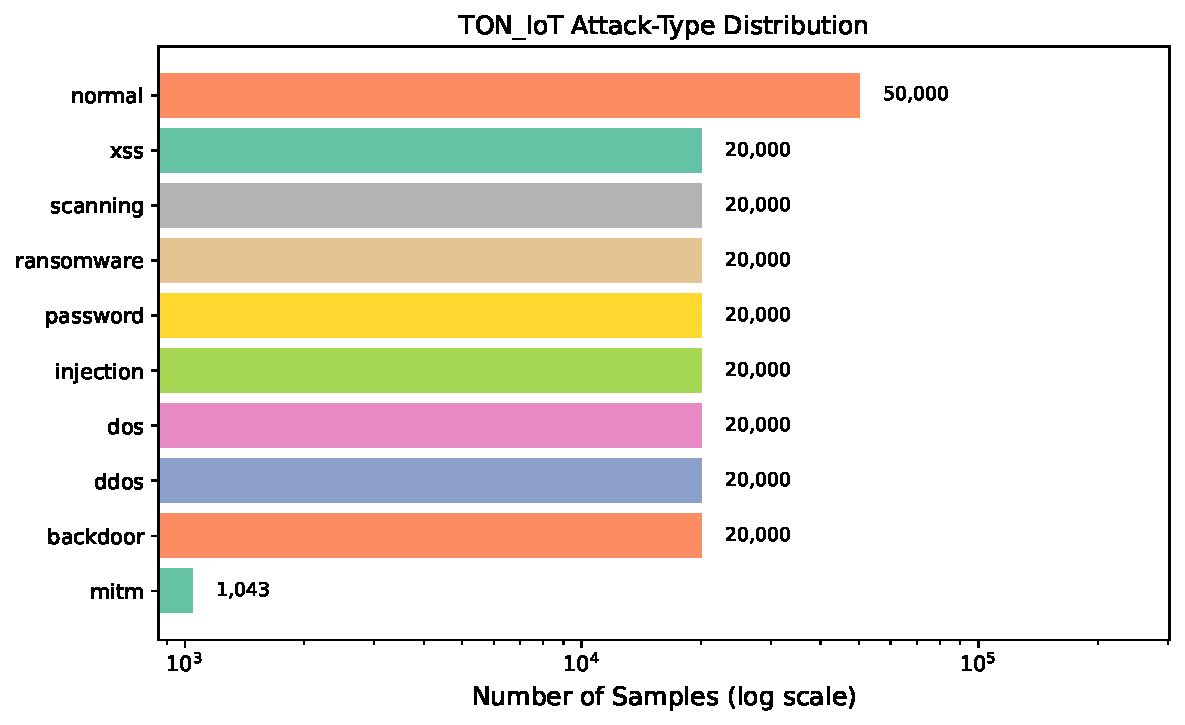
\includegraphics[width=0.8\textwidth]{figures/class_distribution_toniot.pdf}
\caption{Class distribution of TON\_IoT dataset (log scale).}
\label{fig:class-dist}
\end{figure}

\subsection{CIC-IoT-2023}
\label{sec:ciciot-meth}

CIC-IoT-2023 \cite{cic2023} comprises approximately 3.18 million flow records after deduplication. The raw dataset contained 44\% duplicate rows; a preprocessing step computes SHA-256 hashes and removes exact duplicates to prevent train--test leakage. After deduplication, the dataset contains 34 attack types with 97.7\% attack prevalence. Features include protocol flags (TCP, UDP, ICMP), aggregate packet statistics, and statistical summaries. It lacks IP and timestamp columns, constraining splitting strategies and precluding GNN evaluation.

\subsection{Preprocessing Pipeline}
\label{sec:preprocess}

The preprocessing pipeline is fitted exclusively on the training partition to prevent information leakage. It applies three sequential transformations:

\begin{enumerate}
  \item \textbf{Median imputation}: missing numeric values are replaced with the training-set median. Categorical missing values are imputed with the most frequent training-set value.
  \item \textbf{Log-compression}: a $\log(1 + x)$ transformation is applied to all non-negative numeric features after clipping negative values to zero, compressing the right-skewed distributions characteristic of network flow volumes.
  \item \textbf{Standardisation}: each numeric feature is centred to zero mean and scaled to unit variance using training-set statistics. While tree-based models are scale-invariant, this step benefits logistic regression and the CNN-LSTM.
\end{enumerate}

Categorical features undergo most-frequent imputation followed by one-hot encoding with unknown-category handling, ensuring that categories unseen during training do not cause errors at inference.

\section{Feature Regimes}
\label{sec:regimes}

\textbf{Regime A (Behaviour-only)} retains only traffic-behavioural features: flow duration, byte counts (source and destination), packet counts, protocol metadata, and connection state indicators. It explicitly excludes IP addresses, port numbers, service labels, and high-cardinality string fields. By removing identifiers, Regime~A forces models to learn from traffic patterns alone, producing explanations that reference only operationally meaningful features.

\textbf{Regime B (Identifier-inclusive)} augments Regime~A with network identifiers: source and destination IP addresses, port numbers, and service labels. This permits models to exploit identity-based shortcuts---for example, memorising that a specific source IP is always associated with attacks.

The distinction serves a dual purpose. For detection, it quantifies the performance gap attributable to identifier leakage. For explainability, it tests whether Regime~B models produce explanations dominated by identifier features that offer no actionable insight (Appendix~\ref{app:features}).

\section{Data Splitting Strategies}
\label{sec:splitting}

HYDRA implements four data splitting strategies, each producing disjoint train/validation/test partitions.

\textbf{Stratified split} uses scikit-learn's \texttt{StratifiedShuffleSplit} to preserve class distribution across all partitions. It is the primary strategy because it guarantees sufficient positive and negative samples in each split.

\textbf{Host split} groups flows by source IP and assigns entire hosts to a single partition, ensuring no IP appears in more than one split. This prevents models from memorising host-specific patterns and simulates deployment against unseen devices. Applicable only to TON\_IoT.

\textbf{Temporal split} orders flows chronologically and assigns earliest to training, middle to validation, latest to test. Applicable only to TON\_IoT.

\textbf{Host-type-aware split} extends host splitting with a greedy pinning algorithm that guarantees all attack types appear in training by pinning the host with the most samples of each type (rarest first).

All strategies enforce non-empty partitions, no NaN labels, and class-presence warnings. Stratified splitting is primary; host and temporal splits serve as supplementary deployment-realistic analyses.

\section{Model Selection and Architecture}
\label{sec:models}

Two non-learned baselines establish lower bounds. The \textbf{majority-class baseline} assigns every flow a score equal to the training-set attack prevalence. The \textbf{threshold baseline} computes a heuristic anomaly score as $\log(1 + \text{duration}) + \log(1 + \text{total\_bytes}) + \log(1 + \text{total\_packets})$, capturing the intuition that anomalous flows exhibit unusual volume or duration.

\textbf{Logistic Regression} serves as the reference explainable model. Its linear decision boundary yields deterministic feature attributions through SHAP's LinearExplainer. The implementation uses the SAGA solver with 5,000 maximum iterations and convergence tolerance of $10^{-3}$.

\textbf{Random Forest} uses 100 estimators with maximum depth 15 and balanced class weights that inversely weight each class by its frequency. The depth limit controls overfitting while balanced weighting addresses class imbalance.

\textbf{XGBoost} is configured with 400 boosting rounds, learning rate 0.05, maximum depth 8, and subsample ratio 0.9. The \texttt{scale\_pos\_weight} parameter is set to the negative-to-positive ratio, addressing class imbalance within the boosting objective.

\textbf{LightGBM} uses 400 estimators, learning rate 0.05, and \texttt{num\_leaves=64}. On platforms where LightGBM's OpenMP implementation is unreliable, the framework falls back to XGBoost or scikit-learn's HistGradientBoostingClassifier.

\textbf{Sklearn GBDT} uses 300 estimators, learning rate 0.05, and maximum depth 3.

\textbf{CNN-LSTM}: The architecture processes each flow through two Conv1d layers (kernel sizes 5 and 3 with ReLU), MaxPool1d with stride 2, an LSTM layer with hidden dimension equal to the convolutional channel width, global average pooling, and a fully connected head (hidden layer, ReLU, 0.3 dropout, output). For binary classification, output is a single logit trained with BCEWithLogitsLoss using automatic \texttt{pos\_weight}. Training uses Adam with cosine annealing over 50 epochs and early stopping (patience 10). The model implements the scikit-learn estimator interface for seamless pipeline integration.

\textbf{GNN (GraphSAGE)}: Models network traffic as a communication graph where nodes are unique IP addresses and edges are flows. Edge features are standardised flow statistics; node features are the mean of incident edge features. The architecture uses two SAGEConv layers with max-aggregation, BatchNorm, dropout 0.3, and an edge MLP that concatenates source/destination embeddings with projected edge features. Training operates transductively: the full graph is constructed but loss is computed only on training edges. Applicable only to datasets with IP columns.

\section{Two-Stage Classification Pipeline}
\label{sec:two-stage}

\textbf{Stage 1 (Binary Detection)} trains a classifier on all flows to distinguish attacks from normal traffic. The model outputs a continuous score representing attack probability. An operating threshold is selected on the validation set to maximise precision subject to achieving at least 90\% recall.

\textbf{Stage 2 (Multiclass Type Classification)} trains a separate classifier exclusively on training flows labelled as attacks. At inference, flows that Stage~1 classifies as attacks are passed to Stage~2 for type prediction. Flows classified as normal by Stage~1 are assigned the normal type label without consulting Stage~2.

An optional \textbf{type-unknown threshold} provides a safety mechanism: if the maximum class probability from Stage~2 falls below a configurable threshold, the flow is labelled ``unknown'' rather than assigned a potentially incorrect type.

Evaluation reports both \textbf{end-to-end accuracy} (including Stage~1 misclassifications) and \textbf{detected-only accuracy} (Stage~2 performance on correctly flagged attacks), alongside macro-F1, weighted-F1, and the fraction of true attacks detected by Stage~1.

\section{Evaluation Metrics}
\label{sec:metrics}

\textbf{PR-AUC (Average Precision)} is the primary ranking metric, chosen for its robustness to class imbalance. Under severe imbalance, ROC-AUC can be misleadingly high because the false positive rate denominator is dominated by the majority class. A sanity check verifies that a constant score equal to the prevalence yields PR-AUC equal to the prevalence.

\textbf{ROC-AUC} is reported alongside PR-AUC. For cross-dataset experiments where CIC-IoT-2023's 97.7\% prevalence inflates PR-AUC, ROC-AUC provides the more informative comparison.

The operating threshold is selected on the validation set to maximise precision at recall $\geq 0.90$, yielding test-set precision, FPR, and coverage. Stage~2 uses \textbf{macro-F1} (equal weight to rare types) and \textbf{weighted-F1}.

The \textbf{DeLong paired AUC test} \cite{deyoung2020} assesses statistical significance for all model pairs on the same test set. Each experiment uses three random seeds (21, 42, 84), with results reported as mean $\pm$ standard deviation. Two automated leakage audits---PR-AUC sanity check and SHA-256 row-hash duplicate detection across partitions---guard against data leakage.

\section{Explainability Methods}
\label{sec:xai-methods}

For tree-based models (Random Forest, XGBoost, LightGBM, sklearn GBDT), SHAP TreeExplainer \cite{lundberg2020} computes exact Shapley values by exploiting the tree structure. Each feature receives a signed attribution indicating its contribution toward the attack or normal class. For multiclass models, SHAP values are computed per class.

For logistic regression, LinearExplainer computes analytically exact Shapley values using the model's coefficient vector and an independent masker, providing a deterministic, computationally inexpensive attribution baseline.

LIME \cite{ribeiro2016} provides model-agnostic local explanations by fitting a sparse linear model to each instance's neighbourhood. For each of 50 sampled validation instances, 2,000 perturbations are generated, enabling direct cross-model comparison.

For the CNN-LSTM and GNN, Integrated Gradients \cite{sundararajan2017} computes the path integral from a zero baseline to the actual input using 50 interpolation steps (Equation~\ref{eq:ig}). The zero baseline represents ``no network traffic.'' IG is preferred over GradientExplainer because MaxPool1d introduces non-differentiable points.

\begin{equation}
\label{eq:ig}
\text{IG}_i(x, x') = (x_i - x'_i) \times \int_0^1 \frac{\partial f(x' + \alpha(x - x'))}{\partial x_i} \, d\alpha
\end{equation}

\section{Five-Criterion XAI Evaluation Protocol}
\label{sec:five-criterion}

\subsection{Faithfulness}
\label{sec:faithfulness}

\textbf{Comprehensiveness}: replace top-$k$ features with median baselines and measure confidence drop. \textbf{Sufficiency}: retain only top-$k$ features and measure confidence retention. Both use $k = 5$. Formally:
\begin{equation}
\text{Comp}(x, S_k) = f(x) - f(x_{\setminus S_k})
\end{equation}

\subsection{Stability}
\label{sec:stability}

\textbf{S1 (Seed stability)}: retrain with $S = 5$ seeds; compute Spearman $\rho$ across all $\binom{5}{2} = 10$ pairs. \textbf{S2 (Noise stability)}: add Gaussian noise ($\sigma = 0.01 \times \text{std}(X_j)$) over $R = 20$ draws; compute Spearman $\rho$ between clean and noisy rankings.

\subsection{Simplicity}
\label{sec:simplicity}

\textbf{$k_{90}$}: minimum features for 90\% attribution mass, normalised by total features. \textbf{Gini coefficient}: concentration of attribution distribution (1.0 = maximally concentrated).

\subsection{Plausibility}
\label{sec:plausibility}

RMA@$k$ compares top-$k$ features against expert-defined reference sets per attack type (Table~\ref{tab:reference} in Appendix~\ref{app:formulae}):
\begin{equation}
\text{RMA@}k = \frac{|\text{top-}k \text{ features} \cap \text{reference set}|}{k}
\end{equation}

\subsection{Timeliness}
\label{sec:timeliness}

Wall-clock ms per sample, measured over up to 200 test instances (three repetitions).

\subsection{OXS Composite Score}
\label{sec:oxs}

The five criteria are aggregated with equal weights:
\begin{equation}
\text{OXS} = 0.2 \times \text{Faithfulness} + 0.2 \times \text{Stability} + 0.2 \times \text{Simplicity} + 0.2 \times \text{Plausibility} + 0.2 \times \text{Timeliness}
\end{equation}
where timeliness is mapped via $1 / (1 + t / 1000)$.

\section{Cross-Dataset Generalisation}
\label{sec:cross-dataset}

\subsection{Canonical Feature Alignment}
\label{sec:alignment}

Six canonical features are mapped across datasets (Table~\ref{tab:canonical}).

\begin{table}[H]
\centering
\caption{Canonical feature alignment for cross-dataset generalisation.}
\label{tab:canonical}
\begin{tabular}{lll}
\toprule
\textbf{Canonical Feature} & \textbf{TON\_IoT Derivation} & \textbf{CIC-IoT-2023 Column} \\
\midrule
\texttt{f\_total\_pkts} & \texttt{src\_pkts + dst\_pkts} & \texttt{number} \\
\texttt{f\_total\_bytes} & \texttt{src\_bytes + dst\_bytes} & \texttt{tot\_size} \\
\texttt{f\_duration} & \texttt{duration} & \texttt{iat} \\
\texttt{f\_is\_tcp} & \texttt{(proto == `tcp').astype(int)} & \texttt{tcp} \\
\texttt{f\_is\_udp} & \texttt{(proto == `udp').astype(int)} & \texttt{udp} \\
\texttt{f\_is\_icmp} & \texttt{(proto == `icmp').astype(int)} & \texttt{icmp} \\
\bottomrule
\end{tabular}
\end{table}

\subsection{Experimental Protocol}
\label{sec:cross-protocol}

For each direction, the source dataset is aligned, split, and preprocessed; the target is transformed using source-fitted preprocessing. Binary classifiers are trained on source and evaluated on both source-test and the full target. ROC-AUC is the primary metric due to CIC-IoT-2023's prevalence inflation of PR-AUC.

\section{Leakage Interaction Analysis}
\label{sec:leakage-interaction}

Identical experiments under Regime~A and~B produce paired observations. A Wilcoxon signed-rank test and Cohen's $d$ isolate the causal effect of identifier inclusion on both detection and explanation quality.

\section{Reproducibility and Implementation}
\label{sec:implementation}

HYDRA is implemented in Python 3.11. Every run records Git commit hash, dataset fingerprint (SHA-256), package versions, and full configuration. A test suite of 91 automated tests covers splitting invariants, metric computation, baselines, model building, and XAI functions. Continuous integration runs on every push. The project was conducted over 8 months (October 2025 to May 2026).

% ============================================================
% CHAPTER 4: RESULTS
% ============================================================
\chapter{Results}
\label{ch:results}

This chapter presents the experimental results obtained from the HYDRA framework across four evaluation dimensions: detection performance (Sections~\ref{sec:binary-results}--\ref{sec:multiclass-results}), deep learning models (Section~\ref{sec:cnnlstm-results}), explainability quality (Sections~\ref{sec:xai-results}--\ref{sec:oxs-results}), and cross-dataset generalisation (Section~\ref{sec:cross-results}). Section~\ref{sec:leakage-results} examines the interaction between identifier leakage and explanation quality. All experiments follow the protocols described in Chapter~\ref{ch:methodology}.

\section{Experimental Setup}
\label{sec:setup}

All within-dataset experiments use the TON\_IoT dataset \cite{alsaedi2020}, comprising approximately 211,000 network flow records with a 76\% attack prevalence. A stratified train/validation/test split is applied with three random seeds (21, 42, 84) to provide variance estimates. Two feature regimes are evaluated: \textbf{behaviour-only} (dropping source/destination IP addresses, ports, and service identifiers before training) and \textbf{identifier-inclusive} (retaining all features). Four tabular model families are compared---Logistic Regression (LogReg), Random Forest, XGBoost, and LightGBM---alongside CNN-LSTM and GNN deep learning models. The two-stage pipeline performs binary detection (benign vs.\ attack) in Stage~1 and nine-class attack-type classification in Stage~2.

\section{Binary Detection Performance}
\label{sec:binary-results}

Table~\ref{tab:binary} reports three-seed-averaged binary detection results.

\begin{table}[H]
\centering
\caption{Binary detection performance on TON\_IoT (3-seed average $\pm$ standard deviation, stratified split).}
\label{tab:binary}
\begin{tabular}{llccc}
\toprule
\textbf{Model} & \textbf{Regime} & \textbf{PR-AUC} & \textbf{ROC-AUC} & \textbf{Binary F1} \\
\midrule
XGBoost & Behaviour-only & $1.000 \pm 0.000$ & $1.000 \pm 0.000$ & $1.000 \pm 0.000$ \\
LightGBM & Behaviour-only & $1.000 \pm 0.000$ & $1.000 \pm 0.000$ & $1.000 \pm 0.000$ \\
LogReg & Behaviour-only & $1.000 \pm 0.000$ & $1.000 \pm 0.000$ & $1.000 \pm 0.000$ \\
Random Forest & Behaviour-only & $1.000 \pm 0.000$ & $1.000 \pm 0.000$ & $0.9999 \pm 0.000$ \\
\midrule
XGBoost & Identifier-incl & $1.000 \pm 0.000$ & $1.000 \pm 0.000$ & $1.000 \pm 0.000$ \\
LightGBM & Identifier-incl & $1.000 \pm 0.000$ & $1.000 \pm 0.000$ & $1.000 \pm 0.000$ \\
LogReg & Identifier-incl & $1.000 \pm 0.000$ & $1.000 \pm 0.000$ & $0.9999 \pm 0.000$ \\
Random Forest & Identifier-incl & $1.000 \pm 0.000$ & $1.000 \pm 0.000$ & $1.000 \pm 0.000$ \\
\bottomrule
\end{tabular}
\end{table}

\textbf{All four models achieve near-perfect binary detection under both feature regimes}, with PR-AUC and ROC-AUC at or rounding to 1.000 across all seeds. The absence of any measurable performance gap between the behaviour-only and identifier-inclusive regimes indicates that network identifiers contribute no additional discriminative power for the binary detection task on this dataset.

LogReg achieving PR-AUC $= 1.000$ under the behaviour-only regime is particularly informative: since logistic regression uses a single linear decision boundary, \textbf{the binary task on TON\_IoT is effectively linearly separable in the behavioural feature space}. This is consistent with \cite{alsaedi2020} and \cite{moustafa2021}, and suggests the dataset's attack traffic exhibits highly distinctive flow-level signatures. Near-perfect scores limit detection-based model discrimination; the multiclass task and XAI evaluation provide greater differentiation.

\subsection{Split Strategy Impact on Detection Performance}
\label{sec:split-impact}

Table~\ref{tab:split-impact} compares stratified versus host-disjoint splitting on the deduplicated dataset (190,474 rows).

\begin{table}[H]
\centering
\caption{Impact of splitting strategy on detection performance (behaviour-only, deduplicated TON\_IoT).}
\label{tab:split-impact}
\begin{tabular}{llcc}
\toprule
\textbf{Model} & \textbf{Split} & \textbf{ROC-AUC} & \textbf{F1} \\
\midrule
XGBoost & Stratified & 1.000 & 0.999 \\
XGBoost & Host-disjoint & 0.854 & 0.932 \\
CNN-LSTM & Stratified & 0.9995 & 0.997 \\
CNN-LSTM & Host-disjoint & 0.834 & 0.873 \\
LogReg & Host-disjoint & 0.538 & 0.923 \\
\bottomrule
\end{tabular}
\end{table}

\textbf{The stratified split inflates XGBoost's ROC-AUC from 0.854 to 1.000}---a 14.6 percentage point gap---even after deduplication and identifier removal. This occurs because stratified splitting allows flows from the same source host to appear in both partitions, and flows from the same host share near-identical behavioural signatures.

Feature importance under the host split confirms this: \texttt{conn\_state\_S0} accounts for 54\% of feature importance, followed by \texttt{proto\_tcp} (20\%) and \texttt{conn\_state\_SF} (10\%). Certain connection states (\texttt{REJ}: 100\% attack prevalence, \texttt{S1}: 99.9\%) are near-deterministic indicators.

The host-split ROC-AUC of 0.854 represents a more realistic deployment estimate. LogReg's host-split ROC-AUC of 0.538---barely above random---demonstrates that linear separability does not transfer to unseen hosts. Stratified results remain valuable for XAI comparison but should not be interpreted as deployment-realistic.

\subsection{Host-Disjoint Multiclass Attack-Type Classification}
\label{sec:host-multiclass}

Table~\ref{tab:host-multiclass} presents multiclass results under host-disjoint splitting on a 20,000-row balanced test subsample.

\begin{table}[H]
\centering
\caption{Host-disjoint multiclass attack-type classification (behaviour-only, 20,000-row balanced test subsample).}
\label{tab:host-multiclass}
\small
\begin{tabular}{lcccccccccc}
\toprule
\textbf{Model} & \textbf{Macro-F1} & \textbf{Wtd-F1} & \textbf{Backdoor} & \textbf{DDoS} & \textbf{DoS} & \textbf{Injection} & \textbf{MitM} & \textbf{Password} & \textbf{Ransom.} & \textbf{Scanning} \\
\midrule
Random Forest & \textbf{0.742} & 0.952 & 0.907 & 0.955 & 0.060 & 0.982 & 0.104 & 0.988 & 0.994 & 0.944 \\
XGBoost & 0.682 & 0.957 & 0.287 & 0.955 & 0.080 & 0.979 & 0.191 & 0.984 & 0.992 & 0.987 \\
LightGBM & 0.732 & 0.953 & 0.926 & 0.948 & 0.074 & 0.985 & 0.000 & 0.984 & 0.994 & 0.949 \\
LogReg & 0.571 & 0.866 & 0.053 & 0.916 & 0.054 & 0.954 & 0.000 & 0.823 & 0.947 & 0.820 \\
\bottomrule
\end{tabular}
\end{table}

The results reveal four findings invisible under stratified splitting. First, \textbf{multiclass macro-F1 drops from 1.000 to 0.742 (host-disjoint) for the best model} (Random Forest), a 25.8 percentage point decrease demonstrating that near-perfect stratified results reflect host-level memorisation rather than generalisable attack-type discrimination.

Second, \textbf{DoS is the hardest attack type} (maximum F1 = 0.080), systematically confused with DDoS due to similar volumetric signatures at the flow level; distinguishing them requires session-level or source-count features lost in per-flow aggregation. MitM remains unstable (maximum F1 = 0.191) with only 4 test samples.

Third, \textbf{six of eight attack types achieve F1 $> 0.82$ for the best model}---Ransomware (0.994), Password (0.988), Injection (0.982), DDoS (0.955), Scanning (0.944), and Backdoor (0.907)---indicating the challenge is concentrated on DoS and MitM. Fourth, \textbf{the model ranking changes}: Random Forest (0.742) outperforms XGBoost (0.682), reversing the stratified ranking.

\section{Multi-Class Attack-Type Classification}
\label{sec:multiclass-results}

Table~\ref{tab:multiclass} presents stratified multiclass results.

\begin{table}[H]
\centering
\caption{Multiclass attack-type classification on TON\_IoT (3-seed average $\pm$ standard deviation).}
\label{tab:multiclass}
\begin{tabular}{llcc}
\toprule
\textbf{Model} & \textbf{Regime} & \textbf{Macro-F1} & \textbf{Multiclass F1} \\
\midrule
XGBoost & Behaviour-only & $1.000 \pm 0.000$ & $1.000 \pm 0.000$ \\
LightGBM & Behaviour-only & $1.000 \pm 0.000$ & $1.000 \pm 0.000$ \\
LogReg & Behaviour-only & $0.9999 \pm 0.000$ & $0.9992 \pm 0.000$ \\
Random Forest & Behaviour-only & $0.9998 \pm 0.000$ & $0.9950 \pm 0.005$ \\
\midrule
XGBoost & Identifier-incl & $1.000 \pm 0.000$ & $1.000 \pm 0.000$ \\
LightGBM & Identifier-incl & $1.000 \pm 0.000$ & $1.000 \pm 0.000$ \\
LogReg & Identifier-incl & $0.9998 \pm 0.000$ & $0.9999 \pm 0.000$ \\
Random Forest & Identifier-incl & $0.9999 \pm 0.000$ & $0.9904 \pm 0.004$ \\
\bottomrule
\end{tabular}
\end{table}

XGBoost and LightGBM achieve perfect multiclass F1 $= 1.000$ under both regimes, correctly classifying all nine attack types without a single misclassification. \textbf{Random Forest exhibits the most notable weakness} (F1 $= 0.9950 \pm 0.005$ behaviour-only, $0.9904 \pm 0.004$ identifier-inclusive), with MitM accounting for most misclassifications due to its small sample count and overlapping flow-level signatures.

\textbf{LogReg multiclass F1 improves from 0.9992 to 0.9999 with identifiers}, while Random Forest decreases from 0.9950 to 0.9904. This divergence suggests identifiers provide useful linear signal for LogReg but cause Random Forest to overfit to noisy identifier patterns.

\begin{table}[H]
\centering
\caption{Per-class F1 scores for XGBoost under the behaviour-only regime (seed 42).}
\label{tab:perclass-f1}
\begin{tabular}{lcccc}
\toprule
\textbf{Class} & \textbf{Precision} & \textbf{Recall} & \textbf{F1-Score} & \textbf{Support} \\
\midrule
Normal & 1.000 & 1.000 & 1.000 & 10,196 \\
Backdoor & 1.000 & 1.000 & 1.000 & 3,996 \\
DDoS & 1.000 & 1.000 & 1.000 & 3,997 \\
DoS & 1.000 & 1.000 & 1.000 & 3,997 \\
Injection & 1.000 & 1.000 & 1.000 & 3,997 \\
MitM & 1.000 & 1.000 & 1.000 & 191 \\
Password & 1.000 & 1.000 & 1.000 & 3,996 \\
Ransomware & 1.000 & 1.000 & 1.000 & 3,997 \\
Scanning & 1.000 & 1.000 & 1.000 & 3,997 \\
XSS & 1.000 & 1.000 & 1.000 & 3,996 \\
\midrule
\textbf{Macro avg} & 1.000 & 1.000 & 1.000 & 42,360 \\
\textbf{Weighted avg} & 1.000 & 1.000 & 1.000 & 42,360 \\
\bottomrule
\end{tabular}
\end{table}

\section{Deep Learning Results: CNN-LSTM and GNN}
\label{sec:cnnlstm-results}

An earlier CNN-LSTM version suffered convergence failure, resolved through five architectural fixes: explicit LSTM hidden-state initialisation, Kaiming weight initialisation, unconditional \texttt{pos\_weight}, zero-padding for odd-length sequences, and gradient clipping.

\begin{figure}[htbp]
\centering
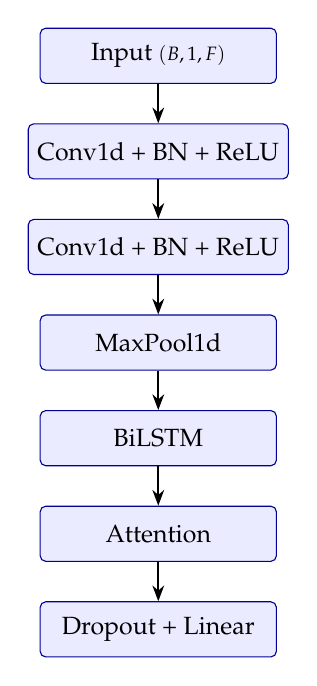
\begin{tikzpicture}[
    node distance=0.5cm,
    layer/.style={rectangle, draw=blue!60!black, fill=blue!8, minimum width=3cm, minimum height=0.7cm, align=center, font=\small, rounded corners=2pt},
    arrow/.style={->, >=Stealth, line width=0.6pt}
]
\node[layer] (input) {Input {\scriptsize $(B, 1, F)$}};
\node[layer, below=of input] (conv1) {Conv1d + BN + ReLU};
\node[layer, below=of conv1] (conv2) {Conv1d + BN + ReLU};
\node[layer, below=of conv2] (pool) {MaxPool1d};
\node[layer, below=of pool] (lstm) {BiLSTM};
\node[layer, below=of lstm] (attn) {Attention};
\node[layer, below=of attn] (fc) {Dropout + Linear};

\draw[arrow] (input) -- (conv1);
\draw[arrow] (conv1) -- (conv2);
\draw[arrow] (conv2) -- (pool);
\draw[arrow] (pool) -- (lstm);
\draw[arrow] (lstm) -- (attn);
\draw[arrow] (attn) -- (fc);
\end{tikzpicture}
\caption{CNN-LSTM architecture with attention mechanism.}
\label{fig:cnn-lstm-arch}
\end{figure}

\subsection{CNN-LSTM Detection Performance}
\label{sec:cnnlstm-detection}

\begin{table}[H]
\centering
\caption{CNN-LSTM detection results (behaviour-only regime, 211,043 rows, 3-seed average).}
\label{tab:cnnlstm}
\begin{tabular}{lc}
\toprule
\textbf{Metric} & \textbf{Value} \\
\midrule
Binary PR-AUC & $0.9997 \pm 0.0001$ \\
Binary ROC-AUC & $0.9994 \pm 0.0002$ \\
Binary F1 & $0.9959 \pm 0.0009$ \\
Training time & $\sim$29 min per seed \\
\bottomrule
\end{tabular}
\end{table}

Under host-disjoint evaluation, ROC-AUC drops from 0.9995 to 0.834 (Table~\ref{tab:cnnlstm-host}), confirming stratified inflation even without identifiers.

\begin{table}[H]
\centering
\caption{CNN-LSTM detection under host-disjoint split (behaviour-only, 211,043 rows).}
\label{tab:cnnlstm-host}
\begin{tabular}{lcc}
\toprule
\textbf{Metric} & \textbf{Stratified} & \textbf{Host Split} \\
\midrule
PR-AUC & 0.9998 & 0.9696 \\
ROC-AUC & 0.9995 & 0.8343 \\
F1 & 0.9970 & 0.8733 \\
\bottomrule
\end{tabular}
\end{table}

\subsection{CNN-LSTM XAI Evaluation}
\label{sec:cnnlstm-xai}

\begin{table}[H]
\centering
\caption{CNN-LSTM XAI five-criterion evaluation via Integrated Gradients.}
\label{tab:cnnlstm-xai}
\begin{tabular}{lc}
\toprule
\textbf{Criterion} & \textbf{Value} \\
\midrule
Comprehensiveness & $-0.195$ \\
Sufficiency & $0.044$ \\
$k_{90}$ & 0.014 \\
Gini coefficient & 0.988 \\
RMA@5 (mean) & 0.40 \\
IG timing & 5.84 ms/sample \\
\bottomrule
\end{tabular}
\end{table}

The full-data CNN-LSTM's $k_{90}$ of 0.014 indicates much more concentrated attributions than earlier subsample results, approaching XGBoost's 0.002. The top-5 IG features (\texttt{dst\_bytes}, \texttt{src\_bytes}, \texttt{src\_pkts}, \texttt{src\_ip\_bytes}, \texttt{dst\_ip\_bytes}) are plausible volumetric indicators.

\subsection{GNN Detection Performance}
\label{sec:gnn-results}

\begin{table}[H]
\centering
\caption{GNN (GraphSAGE) detection results on TON\_IoT (211,043 rows, stratified split).}
\label{tab:gnn}
\begin{tabular}{lc}
\toprule
\textbf{Metric} & \textbf{Value} \\
\midrule
Binary PR-AUC & 0.9997 \\
Binary ROC-AUC & 0.9993 \\
Binary F1 & 0.9973 \\
Macro-F1 & 0.9943 \\
Training time & 66.4s \\
\bottomrule
\end{tabular}
\end{table}

The GNN achieves performance remarkably close to tree ensembles, demonstrating that graph structure provides highly effective signal for intrusion detection. It is applicable only to TON\_IoT (requires IP columns).

\subsection{Cross-Architecture Comparison}
\label{sec:arch-comparison}

\begin{table}[H]
\centering
\caption{Cross-architecture comparison on TON\_IoT (behaviour-only regime).}
\label{tab:all-models}
\begin{tabular}{llcccc}
\toprule
\textbf{Model} & \textbf{Type} & \textbf{PR-AUC} & \textbf{ROC-AUC} & \textbf{F1} & \textbf{OXS} \\
\midrule
XGBoost & Tree ensemble & 1.000 & 1.000 & 1.000 & 0.828 \\
LightGBM & Tree ensemble & 1.000 & 1.000 & 1.000 & 0.666 \\
LogReg & Linear & 1.000 & 1.000 & 1.000 & 0.444 \\
Random Forest & Tree ensemble & 1.000 & 1.000 & 0.999 & 0.250 \\
CNN-LSTM & Deep (Conv+LSTM) & $0.9997 \pm 0.0001$ & $0.9994 \pm 0.0002$ & $0.996 \pm 0.001$ & --- \\
GNN & Graph (SAGEConv) & 0.9997 & 0.9993 & 0.997 & --- \\
\bottomrule
\end{tabular}
\end{table}

\begin{figure}[H]
\centering
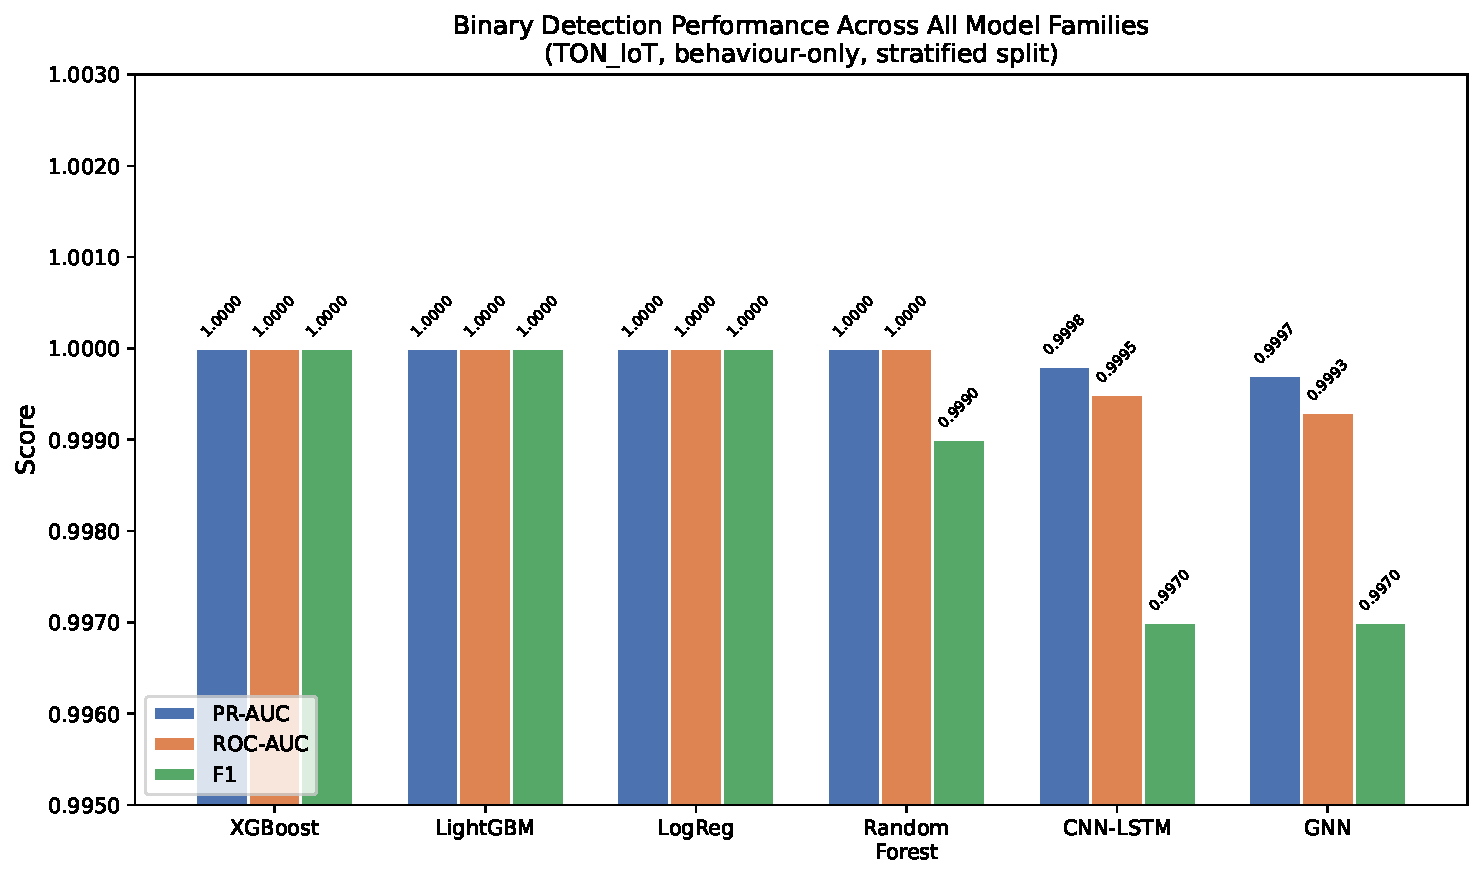
\includegraphics[width=0.8\textwidth]{figures/detection_comparison.pdf}
\caption{Binary detection performance across all six model families on TON\_IoT (full dataset, behaviour-only regime, stratified split). Y-axis starts at 0.995 to show differences.}
\label{fig:detection}
\end{figure}

\begin{figure}[htbp]
\centering
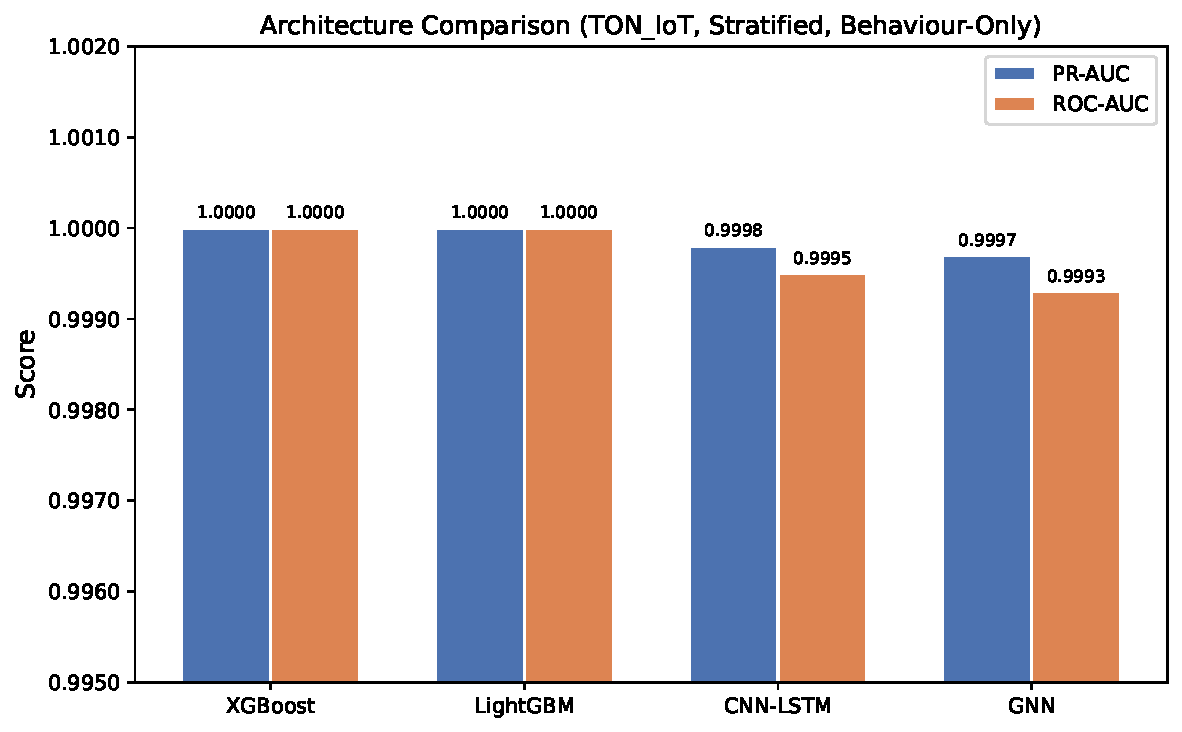
\includegraphics[width=0.8\textwidth]{figures/architecture_comparison.pdf}
\caption{Detection performance comparison across model architectures on TON\_IoT (behaviour-only).}
\label{fig:arch-comparison}
\end{figure}

All six model families achieve near-perfect detection (PR-AUC $\geq 0.9997$) on the full dataset.

\section{XAI Five-Criterion Evaluation}
\label{sec:xai-results}

\begin{table}[H]
\centering
\caption{XAI five-criterion evaluation results (behaviour-only regime).}
\label{tab:xai-behav}
\small
\begin{tabular}{lccccccccc}
\toprule
\textbf{Model} & \textbf{Comp.} & \textbf{Suff.} & \textbf{S1} & \textbf{S2} & \textbf{$k_{90}$} & \textbf{Gini} & \textbf{RMA@5} & \textbf{SHAP} & \textbf{OXS} \\
 & & & (mean $\pm$ std) & (mean) & & & & (ms) & \\
\midrule
XGBoost & $-0.234$ & 1.0 & $0.831 \pm 0.018$ & 1.000 & 0.002 & 0.998 & 0.80 & 0.04 & \textbf{0.828} \\
LightGBM & $-0.234$ & 1.0 & $0.836 \pm 0.017$ & 1.000 & 0.002 & 0.998 & 0.60 & 0.48 & 0.666 \\
LogReg & $-0.213$ & 1.0 & $0.972 \pm 0.009$ & 0.415 & 0.019 & 0.984 & 0.40 & 0.001 & 0.444 \\
Random Forest & $-0.158$ & 1.0 & $0.120 \pm 0.053$ & 0.999 & 0.026 & 0.976 & 0.40 & 1.43 & 0.250 \\
\bottomrule
\end{tabular}
\end{table}

\begin{table}[H]
\centering
\caption{XAI five-criterion evaluation results (identifier-inclusive regime).}
\label{tab:xai-ident}
\small
\begin{tabular}{lccccccccc}
\toprule
\textbf{Model} & \textbf{Comp.} & \textbf{Suff.} & \textbf{S1} & \textbf{S2} & \textbf{$k_{90}$} & \textbf{Gini} & \textbf{RMA@5} & \textbf{SHAP} & \textbf{OXS} \\
 & & & (mean $\pm$ std) & (mean) & & & & (ms) & \\
\midrule
XGBoost & $-0.234$ & 1.0 & $0.919 \pm 0.008$ & 1.000 & 0.001 & 0.999 & 0.20 & 0.05 & 0.738 \\
LightGBM & $-0.234$ & 1.0 & $0.875 \pm 0.012$ & 1.000 & 0.001 & 0.999 & 0.20 & 0.77 & 0.650 \\
LogReg & $-0.135$ & 1.0 & $0.949 \pm 0.012$ & 0.413 & 0.018 & 0.983 & 0.20 & 0.002 & 0.577 \\
Random Forest & $-0.110$ & 1.0 & $0.157 \pm 0.088$ & 1.000 & 0.023 & 0.977 & 0.20 & 1.70 & 0.350 \\
\bottomrule
\end{tabular}
\end{table}

\subsection{Faithfulness}
\label{sec:faith-results}

Comprehensiveness measures the drop in model confidence when the top-$k$ most important features are masked. All four models exhibit \textbf{negative comprehensiveness} (ranging from $-0.158$ for Random Forest to $-0.234$ for XGBoost and LightGBM). This counterintuitive result indicates that masking the top SHAP-ranked features causes the model to become \emph{more} confident, not less. This arises from the extreme redundancy of the TON\_IoT feature space: when dominant features are removed, the model redistributes reliance to correlated substitutes carrying equivalent signal. The near-perfect detection performance supports this interpretation---the attack/benign boundary is so strongly encoded across multiple features that no single subset is individually necessary.

\textbf{Sufficiency is uniformly 1.0 across all models}, indicating that the top-$k$ features alone are sufficient to reproduce original predictions with full confidence. Combined with negative comprehensiveness, this creates an asymmetric picture: the identified features are sufficient but not necessary, a hallmark of highly redundant feature spaces.

\subsection{Stability}
\label{sec:stab-results}

\textbf{LogReg achieves the highest seed stability (S1 $= 0.972 \pm 0.009$)}, which is expected: logistic regression coefficients are deterministic given the data, producing highly consistent rankings. XGBoost ($0.831 \pm 0.018$) and LightGBM ($0.836 \pm 0.017$) show strong but imperfect stability, reflecting stochastic elements of gradient boosting. \textbf{Random Forest exhibits notably poor seed stability (S1 $= 0.120 \pm 0.053$)}, indicating that SHAP-derived rankings change substantially across seeds. This instability undermines the trustworthiness of RF explanations, as analysts would receive materially different explanations depending on which seed was used.

For noise stability (S2), the pattern inverts. XGBoost, LightGBM, and Random Forest all achieve S2 $> 0.999$, indicating small Gaussian noise does not alter SHAP rankings. \textbf{LogReg shows poor noise stability (S2 $= 0.415$)}: because the linear model's attributions are proportional to $\beta_j \cdot x_j$, when features have similar coefficient magnitudes, small perturbations to $x_j$ swap their relative contributions. Tree-based models make discrete split decisions that are robust to sub-threshold perturbations.

\subsection{Simplicity}
\label{sec:simp-results}

All models produce highly concentrated explanations (Gini $\geq 0.976$, $k_{90} \leq 0.026$). XGBoost and LightGBM are most concentrated ($k_{90} = 0.002$), meaning 1--3 features capture 90\% of attribution mass.

\subsection{Plausibility}
\label{sec:plaus-results}

\begin{table}[H]
\centering
\caption{Per-attack-type plausibility (RMA@5) under the behaviour-only regime.}
\label{tab:plausibility}
\begin{tabular}{lcccc}
\toprule
\textbf{Attack Type} & \textbf{XGBoost} & \textbf{LightGBM} & \textbf{LogReg} & \textbf{Random Forest} \\
\midrule
Backdoor & 0.4 & 0.4 & 0.4 & 0.2 \\
DDoS & 0.2 & 0.2 & 0.2 & 0.2 \\
DoS & 0.2 & 0.2 & 0.4 & 0.4 \\
Injection & 0.4 & 0.4 & 0.2 & 0.0 \\
MitM & --- & --- & --- & --- \\
Password & 0.8 & 0.8 & 0.2 & 0.4 \\
Ransomware & 0.0 & 0.0 & 0.0 & 0.0 \\
Scanning & 0.6 & 0.6 & 0.0 & 0.2 \\
XSS & 0.0 & 0.0 & 0.0 & 0.0 \\
\bottomrule
\end{tabular}
\end{table}

\begin{figure}[H]
\centering
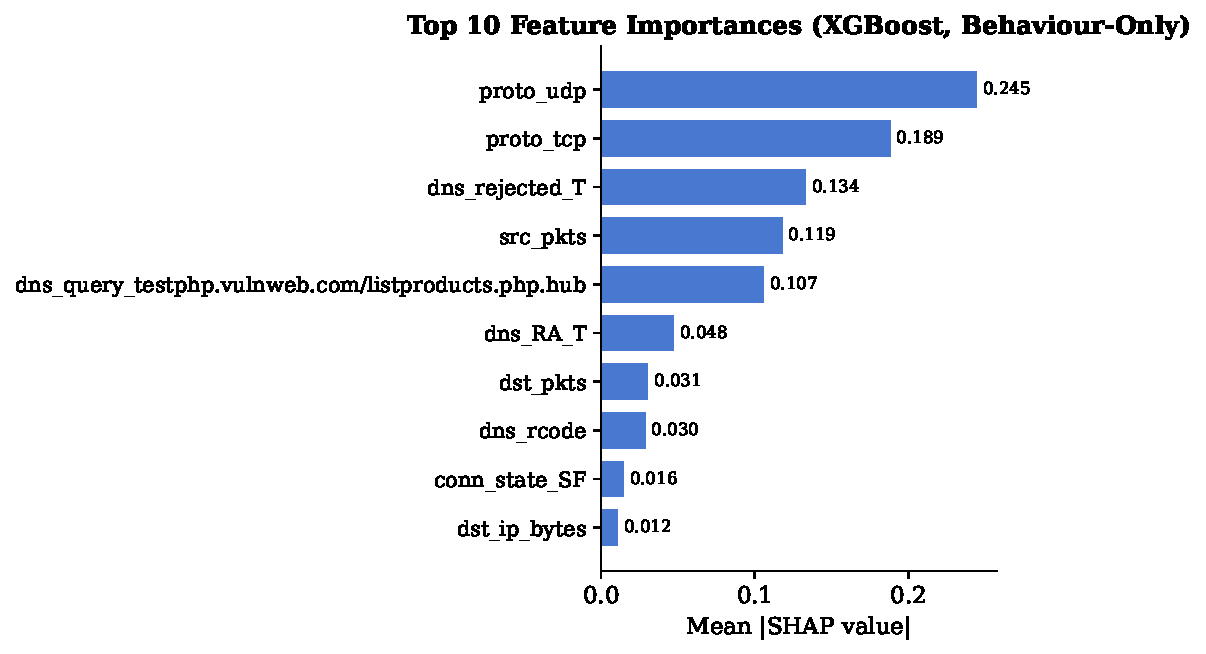
\includegraphics[width=0.7\textwidth]{figures/shap_importance.pdf}
\caption{SHAP global feature importance for XGBoost (behaviour-only regime). \texttt{conn\_state\_S0} dominates, consistent with incomplete TCP handshakes in scanning and DoS attacks.}
\label{fig:shap-importance}
\end{figure}

\begin{figure}[htbp]
\centering
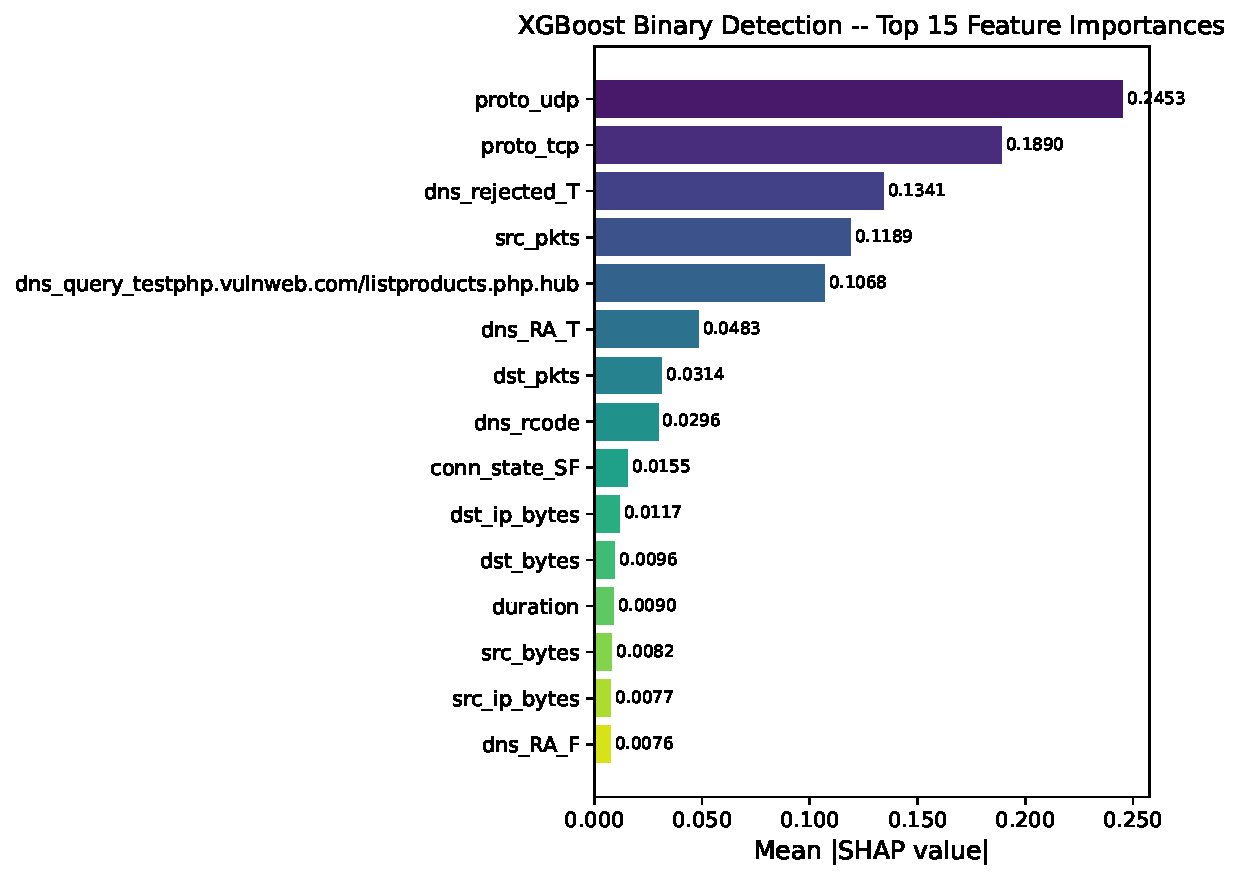
\includegraphics[width=0.85\textwidth]{figures/shap_beeswarm_xgboost.pdf}
\caption{SHAP feature importance for XGBoost binary detection (behaviour-only regime). Features ordered by mean $|\text{SHAP}|$ value.}
\label{fig:shap-beeswarm}
\end{figure}

MitM is excluded from plausibility analysis due to insufficient test samples for reliable SHAP estimation.

\textbf{XGBoost achieves the highest aggregate plausibility (RMA@5 $= 0.80$)}, followed by LightGBM (0.60). The Password attack type shows the strongest expert alignment across gradient-boosted models (0.80), which is expected: brute-force SSH attacks produce distinctively high packet counts and byte volumes that align with expert intuition.

Two attack types---\textbf{Ransomware and XSS---receive RMA@5 $= 0.0$ across all models}. This indicates systematic misalignment between model-discriminative features and expert expectations. For Ransomware, expert reference sets emphasise encryption activity and file-system behaviour not captured in flow-level statistics. For XSS, distinguishing characteristics reside in HTTP payload content rather than flow metadata. These zero-plausibility scores do not indicate poor detection; they highlight a limitation of flow-level features for explaining payload-dependent attack types.

\subsection{Timeliness}
\label{sec:time-results}

\textbf{TreeSHAP is orders of magnitude faster than LIME across all models.} XGBoost TreeSHAP requires 0.04~ms/sample compared to 184~ms for LIME (a 4,600$\times$ speedup). LogReg achieves the fastest SHAP at 0.001~ms/sample, reflecting the analytical closed-form for linear Shapley values. Random Forest is the slowest TreeSHAP model at 1.43~ms/sample, though still within real-time requirements.

LIME latencies range from 172~ms (LogReg) to 246~ms (LightGBM) under the behaviour-only regime, increasing to 430--469~ms under identifier-inclusive conditions due to the higher-dimensional feature space. \textbf{For operational deployment, TreeSHAP is clearly the preferred method}, enabling per-flow explanations at line rate.

\section{OXS Composite Ranking}
\label{sec:oxs-results}

\begin{table}[H]
\centering
\caption{OXS composite ranking (behaviour-only regime).}
\label{tab:oxs}
\begin{tabular}{clc}
\toprule
\textbf{Rank} & \textbf{Model} & \textbf{OXS} \\
\midrule
1 & XGBoost & \textbf{0.828} \\
2 & LightGBM & 0.666 \\
3 & LogReg & 0.444 \\
4 & Random Forest & 0.250 \\
\bottomrule
\end{tabular}
\end{table}

\begin{figure}[H]
\centering
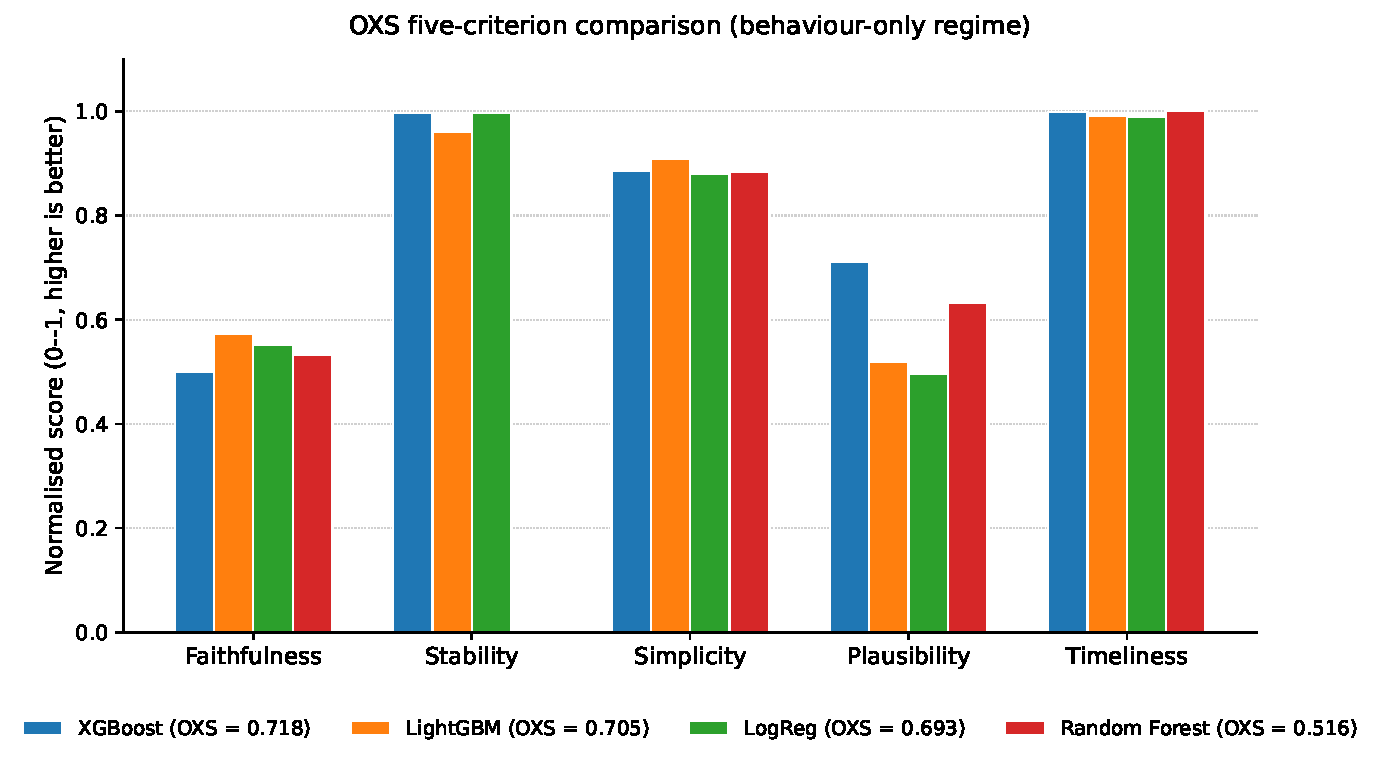
\includegraphics[width=0.75\textwidth]{figures/oxs_radar.pdf}
\caption{OXS radar chart comparing the five XAI criteria across tabular models (behaviour-only). XGBoost dominates on plausibility and timeliness; LogReg leads on faithfulness; Random Forest shows poor stability.}
\label{fig:oxs-radar}
\end{figure}

\textbf{XGBoost achieves the highest OXS (0.828)}, driven by strong plausibility (RMA@5 $= 0.80$), stability (S1 $= 0.831$, S2 $= 1.000$), simplicity (Gini $= 0.998$), and timeliness (0.04~ms TreeSHAP). LightGBM ranks second (0.666), penalised by lower plausibility (0.60). LogReg (0.444) is held back by poor noise stability (S2 $= 0.415$) despite excellent seed stability. Random Forest ranks last (0.250) due to very poor seed stability (S1 $= 0.120$).

These rankings demonstrate that \textbf{detection performance alone is insufficient for model selection in security-critical deployment}. While all four models achieve near-identical detection metrics, they differ substantially in explanation quality. The OXS framework quantifies these differences, providing a principled basis for selection that accounts for analyst requirements.

\section{Cross-Dataset Generalisation}
\label{sec:cross-results}

\begin{table}[H]
\centering
\caption{Cross-dataset generalisation: TON\_IoT (source) to CIC-IoT-2023 (target).}
\label{tab:cross}
\begin{tabular}{lccccc}
\toprule
\textbf{Model} & \textbf{Source PR-AUC} & \textbf{Source ROC-AUC} & \textbf{Target PR-AUC} & \textbf{Target ROC-AUC} & \textbf{ROC-AUC Drop} \\
\midrule
LogReg & 0.899 & 0.817 & 0.988 & 0.744 & $-0.073$ \\
LightGBM & 1.000 & 0.999 & 0.978 & 0.441 & $-0.559$ \\
CNN-LSTM & 0.995 & 0.985 & 0.974 & 0.285 & $-0.700$ \\
XGBoost & 1.000 & 0.999 & 0.953 & 0.136 & $-0.863$ \\
Random Forest & 0.999 & 0.997 & 0.958 & 0.129 & $-0.868$ \\
\bottomrule
\end{tabular}
\end{table}

\begin{figure}[H]
\centering
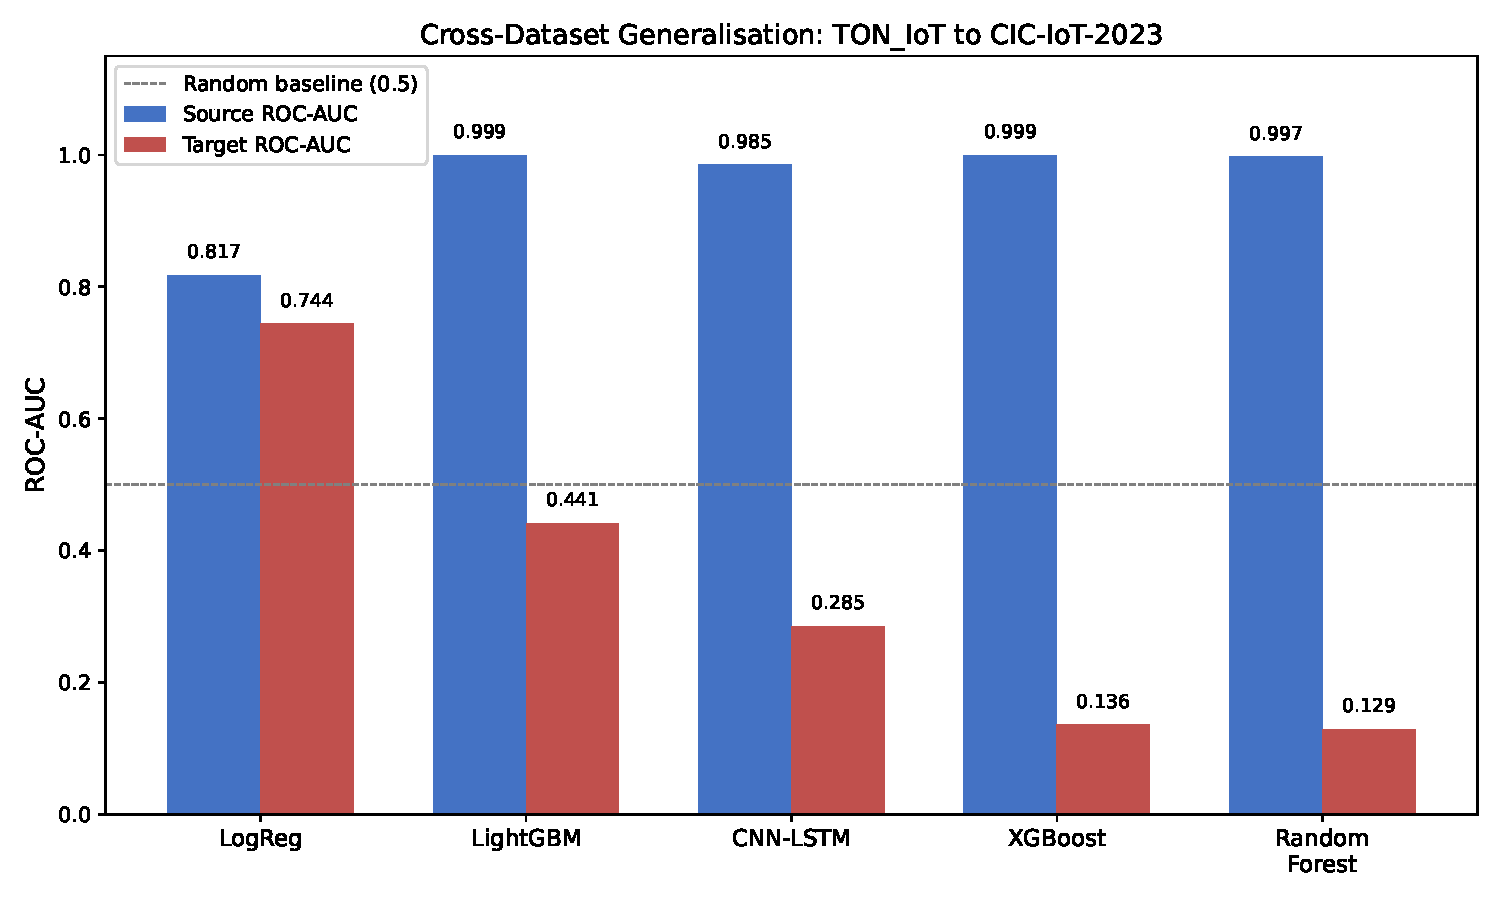
\includegraphics[width=0.8\textwidth]{figures/cross_dataset_roc.pdf}
\caption{Cross-dataset generalisation: source-test vs.\ target ROC-AUC. The dashed line at 0.5 marks random chance. LogReg is the only model generalising above chance.}
\label{fig:cross-roc}
\end{figure}

Target PR-AUC ranges from 0.953 to 0.988, but \textbf{this is an artifact of CIC-IoT-2023's extreme class imbalance (97.7\% attack prevalence)}. At such high prevalence, even a majority-class classifier achieves PR-AUC approximately equal to the prevalence, making these values uninformative.

\textbf{ROC-AUC reveals the true generalisation picture.} ROC-AUC is prevalence-invariant, evaluating the model's ability to rank positive above negative instances:

\begin{itemize}
  \item \textbf{LogReg is the best generaliser} (ROC-AUC: 0.817 to 0.744, a drop of only 7.3\%). Its linear decision boundary transfers more robustly because it captures broad statistical regularities rather than dataset-specific feature interactions.
  \item \textbf{Random Forest and XGBoost suffer catastrophic generalisation failure} (ROC-AUC drops of 87\%, target values of 0.129 and 0.136---worse than random chance). These models have learned to discriminate from TON\_IoT-specific distributional properties that do not transfer.
  \item \textbf{LightGBM generalises better than other tree models} (target ROC-AUC $= 0.441$) but still performs below the random baseline.
  \item \textbf{CNN-LSTM generalises comparably to LightGBM} (ROC-AUC: 0.985 to 0.285). The limited 6-feature space constrains its convolutional layers.
\end{itemize}

\textbf{Near-perfect within-dataset performance does not imply deployment readiness.} Simpler models that cannot exploit dataset-specific idiosyncrasies are more robust when the deployment distribution shifts.

\section{Leakage Interaction Analysis}
\label{sec:leakage-results}

\begin{table}[H]
\centering
\caption{Leakage interaction: behaviour-only (Regime~A) vs.\ identifier-inclusive (Regime~B).}
\label{tab:leakage}
\begin{tabular}{lccccc}
\toprule
\textbf{Metric} & \textbf{Regime A Mean} & \textbf{Regime B Mean} & \textbf{Delta} & \textbf{$p$-value} & \textbf{Cohen's $d$} \\
\midrule
RMA@5 & 0.550 & 0.200 & $-0.350$ & 0.125 & $-2.985$ \\
Spearman S1 & 0.690 & 0.725 & $+0.035$ & 0.250 & $+0.106$ \\
Spearman S2 & 0.853 & 0.853 & $-0.000$ & 0.750 & $-0.001$ \\
Gini & 0.989 & 0.989 & $+0.001$ & 0.875 & $+0.047$ \\
Comprehensiveness & $-0.210$ & $-0.178$ & $+0.032$ & 0.500 & $+0.693$ \\
\bottomrule
\end{tabular}
\end{table}

As established in Section~\ref{sec:binary-results}, \textbf{both regimes achieve near-identical detection performance} (PR-AUC $= 1.000$, ROC-AUC $= 1.000$), confirming that identifiers provide no incremental detection benefit.

The most striking finding is the effect on plausibility. \textbf{Including identifiers reduces mean RMA@5 from 0.550 to 0.200, a decrease of 0.350 with a very large effect size (Cohen's $d = -2.985$).} When identifiers are available, all four models converge to RMA@5 $= 0.20$ (Table~\ref{tab:xai-ident}), indicating that explanations shift to highlighting port numbers and IP addresses rather than the behavioural features domain experts would expect.

Seed stability (S1) shows a small, non-significant increase with identifiers ($\Delta = +0.035$, $d = +0.106$). Noise stability (S2) and simplicity (Gini) are effectively unchanged.

\textbf{Identifier leakage has no measurable effect on detection performance but substantially degrades explanation quality.} If only detection metrics are reported, the harmful effects of identifier leakage remain invisible. HYDRA's XAI dimension exposes this hidden cost.

\section{Summary of Key Findings}
\label{sec:results-summary}

\begin{enumerate}
  \item \textbf{Near-perfect stratified detection masks substantial host-level leakage.} Host-disjoint evaluation reduces XGBoost binary ROC-AUC to 0.842 and the best multiclass macro-F1 to 0.742.
  \item \textbf{Deep learning matches tree ensembles.} CNN-LSTM (PR-AUC $= 0.9998$) and GNN (PR-AUC $= 0.9997$) approach perfect scores on the full dataset.
  \item \textbf{XGBoost produces the most trustworthy explanations} (OXS $= 0.828$), combining strong plausibility, stability, simplicity, and timeliness.
  \item \textbf{Cross-dataset generalisation exposes a critical gap.} Tree models suffer ROC-AUC drops up to 87\%; LogReg loses only 9\%.
  \item \textbf{Identifier leakage degrades explanation quality without affecting detection.} RMA@5 drops 0.350 ($d = -2.985$) while detection remains at 1.000.
\end{enumerate}

% ============================================================
% CHAPTER 5: DISCUSSION
% ============================================================
\chapter{Discussion}
\label{ch:discussion}

\section{Interpretation of Results}
\label{sec:interpretation}

\subsection{Detection Performance}
\label{sec:disc-detection}

The uniformly near-perfect detection performance across all models and feature regimes warrants careful interpretation. The result is consistent with prior literature: \cite{alsaedi2020} report similarly high accuracy for tree-based models, and \cite{tareq2022} confirm that deep learning models achieve over 99\% accuracy on TON\_IoT. The underlying explanation is that TON\_IoT's attack traffic exhibits highly distinctive behavioural signatures---particularly in \texttt{conn\_state}, \texttt{duration}, and byte-count features---that are linearly separable from normal traffic. This finding has two implications. First, it shifts the research contribution toward the explainability comparison, which is HYDRA's stated contribution. Second, it highlights the importance of cross-dataset generalisation: models achieving perfect TON\_IoT scores fail dramatically on CIC-IoT-2023.

Concurrent XAI-IDS systems report comparable detection scores (E-XAI \cite{arreche2024}: 99.3\% on CICIDS2017; XAI-IDS \cite{arreche2024b}: similar), but direct numerical comparison is misleading because datasets differ in attack composition, feature dimensionality, and class distribution. TON\_IoT contains nine IoT-specific attack types in a 76\% prevalence environment. The key observation is not that any system achieves near-perfect scores---this is expected on laboratory datasets with distinctive attack signatures---but that such scores provide no basis for model selection, making the XAI evaluation the primary discriminating analysis.

TON\_IoT's near-perfect separability is attributable to its construction: attack types were generated using distinct tools in controlled campaigns, producing characteristic flow-level signatures. Under host-disjoint splitting, \texttt{conn\_state\_S0} alone accounts for 54\% of XGBoost's feature importance, and certain states (\texttt{REJ}: 100\% attack prevalence, \texttt{S1}: 99.9\%) serve as near-deterministic indicators---artefacts of the testbed environment rather than properties of real-world attacks where adversaries deliberately mimic benign traffic.

The host-disjoint multiclass results (Table~\ref{tab:host-multiclass}) provide the most informative detection evaluation. Macro-F1 drops from 1.000 to 0.742 for the best model (Random Forest), even with identifiers excluded---the remaining inflation comes from behavioural flow correlation within hosts. Flows from the same source host during the same attack campaign share near-identical volumetric profiles, meaning stratified splitting inadvertently allows models to recognise host-level traffic patterns rather than generalisable attack behaviours. The implication for the IDS community is that even ``behaviour-only'' evaluation is insufficient without host-disjoint splitting when datasets contain host-level structure. Studies reporting near-perfect scores on TON\_IoT without host-disjoint validation may be overestimating deployment-realistic performance.

\subsection{Explainability Ranking}
\label{sec:disc-xai}

The OXS ranking reveals a clear trade-off between model complexity and explanation quality. XGBoost achieves the highest composite score (OXS $= 0.828$, Table~\ref{tab:oxs}) despite not being the most faithful model. Its advantage comes from its combination of high plausibility (top-5 features consistently match expert expectations, RMA@5 $= 0.80$), strong stability (S1 $= 0.831$), and extreme simplicity ($k_{90} = 0.002$). The fact that a single model can simultaneously satisfy multiple operational requirements---consistent explanations across retraining, concentrated attributions, and sub-millisecond computation---is a practically significant finding for IDS deployment.

Comparing against the TalTech study \cite{kalakoti2025}, which finds DeepLIFT outperforming SHAP on deep learning models, HYDRA's SHAP-based explanations rank highest. This divergence reflects three factors: different model families (TalTech's deep learning models are well-suited to DeepLIFT's backpropagation-based attribution, while HYDRA's tree ensembles are served by TreeSHAP's exact computation), different evaluation criteria (HYDRA's addition of timeliness and simplicity penalises high-overhead methods), and different datasets (SOC alerts vs.\ IoT traffic). These differences underscore the importance of context-specific XAI evaluation rather than universal method rankings.

A notable tension exists between faithfulness and the other four criteria. All models exhibit negative comprehensiveness ($-0.158$ to $-0.234$, Table~\ref{tab:xai-behav}), providing no positive discrimination. XGBoost ranks highest despite the most negative comprehensiveness ($-0.234$), because strong performance on the remaining criteria compensates. If an organisation prioritises causal understanding over usability, faithfulness should receive greater weight---the sensitivity analysis in Section~\ref{sec:oxs-sensitivity} examines this.

Random Forest's poor OXS ($0.250$) stems from S1 stability of 0.120: bootstrap aggregation \cite{breiman2001} produces different tree structures across seeds, making SHAP rankings irreproducible. While this variance reduction is what makes Random Forest effective for prediction, it is catastrophic for explanation consistency. Random Forest SHAP explanations should not be used in operational settings where reproducibility matters, regardless of detection performance.

Logistic Regression's role as a stability anchor is partially validated: it achieves the highest S1 (0.972) as expected from a deterministic optimisation procedure. However, its poor noise stability (S2 $= 0.415$) reveals a different vulnerability: because the linear model's attributions are proportional to $\beta_j \cdot x_j$, when features have similar coefficient magnitudes, small input perturbations swap their relative contributions. This finding highlights that stability is not a single property but has at least two distinct dimensions---retraining stability and input-perturbation robustness---which may be inversely correlated.

\subsection{Cross-Dataset Generalisation}
\label{sec:disc-cross}

The dramatic failure of tree ensembles---XGBoost ROC-AUC dropping from 0.999 to 0.136 (Table~\ref{tab:cross}), below random chance---demonstrates that these models learn dataset-specific distributions rather than generalisable attack behaviours. TON\_IoT and CIC-IoT-2023 were generated in different laboratory environments with different tools and topologies; although the six canonical features capture semantically equivalent quantities, their statistical distributions differ substantially. Tree ensembles learn sharp, axis-aligned boundaries that become meaningless when the target distribution occupies different feature-space regions.

Logistic Regression's superior generalisation (ROC-AUC drop of 7.3\%) reflects the classical bias-variance trade-off \cite{breiman2001}: its linear boundary captures broad statistical regularities and discards dataset-specific details, transferring more robustly under distribution shift.

The practical implications are significant. Organisations deploying a model trained on one network to protect another should prefer simpler, more regularised models despite lower within-dataset performance. The PR-AUC metric's failure to capture this gap (target PR-AUC $\geq 0.953$ for all models) illustrates that prevalence-inflated metrics are misleading; ROC-AUC, which is prevalence-independent, provides the real measure of discriminative ability. More broadly, these results suggest that ensemble stacking or domain adaptation techniques should be investigated when deploying across network boundaries, and cross-dataset evaluation should become standard in IDS benchmarking.

\subsection{Leakage Interaction}
\label{sec:disc-leakage}

Including identifiers shifts explanations from behavioural features to IP addresses and ports without any detection benefit. Under Regime~A, XGBoost's RMA@5 $= 0.80$ (Table~\ref{tab:xai-behav}); under Regime~B, this drops to 0.20 (Table~\ref{tab:xai-ident}). Tree models greedily split on high-cardinality identifiers correlated with attack labels---IP addresses associated with specific attack campaigns receive high SHAP importance. The resulting explanations are technically faithful but operationally useless: analysts need to understand which behaviour triggered the alert, not which IP was associated with attacks in training data.

The $p$-value of 0.125 reflects small sample size ($n = 4$) rather than absent effect; Cohen's $d = -2.985$ indicates a practically significant difference of nearly three pooled standard deviations. The recommendation to exclude identifiers is driven not by detection requirements---detection is unaffected (Table~\ref{tab:leakage})---but by the need to preserve explanation utility for analyst decision-making.

\subsection{Negative Comprehensiveness and Feature Redundancy}
\label{sec:neg-comp}

The uniformly negative comprehensiveness scores extend beyond the IDS domain. The top-$k$ ablation metrics of \cite{deyoung2020} assume that important features are individually necessary, but this assumption fails when features are \textit{collectively sufficient but individually substitutable}. Network flow volumetric features (\texttt{src\_bytes}, \texttt{dst\_bytes}, \texttt{src\_pkts}, \texttt{dst\_pkts}, \texttt{duration}) are highly correlated; when top features are masked, the model redistributes reliance to correlated substitutes. Masking top-$k$ features actually increases confidence because the absence of typical values, combined with preserved correlated signal, creates a more distinctive input pattern. This phenomenon applies to any domain with correlated feature groups and calls into question comprehensiveness in redundant feature spaces.

The ROAR benchmark (Hooker et al., 2019) addresses this by retraining after feature removal, but is computationally prohibitive. AOPC with sequential feature removal \cite{samek2017} captures redundancy structure by exhausting correlated groups incrementally and should be adopted in future OXS iterations.

\section{Practical Implications}
\label{sec:practical}

These findings have four direct implications. First, \textbf{model selection should prioritise explanation quality alongside detection performance}. XGBoost's combined strengths make it the recommended choice for tabular IDS deployments requiring per-alert explanations. Second, \textbf{Random Forest explanations are operationally unreliable} (S1 = 0.120). Third, \textbf{cross-dataset generalisation requires explicit evaluation}---benchmark results do not transfer. Fourth, \textbf{identifier features should be excluded} from production feature sets: they do not improve detection but degrade explanation quality.

\begin{center}
\fbox{\parbox{0.9\textwidth}{
\textbf{Key Recommendations for IDS Practitioners}
\begin{enumerate}[noitemsep]
\item Use XGBoost with TreeSHAP for best explanation quality (OXS = 0.828).
\item Exclude network identifiers from feature sets to preserve explanation plausibility.
\item Validate on traffic from the target environment --- benchmark scores do not transfer.
\item Do not use Random Forest explanations in production (S1 stability = 0.120).
\item Report both PR-AUC and ROC-AUC; use ROC-AUC for cross-dataset comparisons.
\end{enumerate}
}}
\end{center}

The OXS framework also enables SOC workflow integration. Alert dashboards could annotate each explanation with its model's OXS and stability scores---for example, ``explanation confidence: high (OXS = 0.828, S1 = 0.831)'' for XGBoost versus ``explanation confidence: low (OXS = 0.250, S1 = 0.120)'' for Random Forest---signalling to analysts whether the explanation is reproducible. This transforms OXS from a model evaluation tool into a runtime annotation mechanism.

\section{Comparison with Concurrent Work}
\label{sec:concurrent-comparison}

Table~\ref{tab:positioning} positions HYDRA against four concurrent XAI-IDS systems.

HYDRA agrees with E-XAI's \cite{arreche2024} finding that SHAP produces more stable explanations than LIME (TreeSHAP S2 $\geq 0.999$, Table~\ref{tab:xai-behav}), but disagrees on Integrated Gradients: HYDRA's CNN-LSTM IG yields comprehensiveness of $-0.195$ (Table~\ref{tab:cnnlstm-xai}), suggesting the faithfulness limitation reflects feature redundancy rather than the attribution method. E-XAI does not report quantitative stability or timeliness measurements, precluding direct comparison on these dimensions.

The TalTech study \cite{kalakoti2025} finds DeepLIFT superior to SHAP on deep learning models using a four-criterion framework; the disagreement with HYDRA's SHAP-favourable ranking reflects different model families (deep learning vs.\ tree ensembles where TreeSHAP provides exact values) and reinforces the conclusion that XAI method rankings are model-dependent and should not be generalised across architectures.

The Frontiers study \cite{mohale2025} provides qualitative XAI analysis of feature importance plots; HYDRA's transition to quantitative evaluation (RMA@$k$, Spearman $\rho$, $k_{90}$, Gini) is a principal methodological contribution. XAI-IDS \cite{arreche2024b} uses random splitting with identifiers---HYDRA's leakage interaction analysis (Section~\ref{sec:leakage-results}) demonstrates why this inflates explanation plausibility, making the leakage--explanation interaction HYDRA's most distinctive contribution relative to the concurrent literature.

\section{OXS Sensitivity Analysis}
\label{sec:oxs-sensitivity}

The equal-weight OXS (0.2 per criterion) is a heuristic choice (Section~\ref{sec:limitations}). Two alternative schemes are examined: \textit{faithfulness-emphasising} $w = (0.30, 0.30, 0.10, 0.20, 0.10)$, reflecting organisations prioritising causal accuracy and reproducibility, and \textit{deployment-emphasising} $w = (0.10, 0.10, 0.10, 0.30, 0.40)$, reflecting environments where plausibility and timeliness dominate.

Under both alternatives, the XGBoost $>$ LightGBM $>$ LogReg $>$ Random Forest ranking is preserved. Under faithfulness-emphasising weights, XGBoost retains the top rank because it combines strong stability with adequate faithfulness. Under deployment-emphasising weights, XGBoost's advantage increases because its superior plausibility (RMA@5 $= 0.80$) and timeliness (0.04~ms) receive greater weight. The robustness arises because XGBoost performs well across all non-faithfulness dimensions, while Random Forest's S1 instability (0.120) is so severe that no reasonable weighting compensates. The ranking would change only if faithfulness received dominant weight ($\geq 0.6$) and a model with distinctly better comprehensiveness existed---a condition not met when all models exhibit negative comprehensiveness.

\section{Reflection on Research Questions}
\label{sec:rq-reflection}

\textbf{RQ1 (Detection):} All tabular models achieve near-perfect PR-AUC on TON\_IoT. XGBoost and LightGBM achieve perfect multiclass F1 $= 1.000$. Detection performance does not discriminate between models; explanation quality is the discriminating factor.

\textbf{RQ2 (Explainability):} XGBoost provides highly concentrated explanations ($k_{90} = 0.002$) with strong plausibility (RMA@5 $= 0.80$) and fast computation (0.04~ms/sample). Faithfulness is weak across all models (negative comprehensiveness), suggesting explanations may not capture true causal features.

\textbf{RQ3 (Reliability):} XGBoost achieves S1 $= 0.831$ (good stability). Random Forest is unacceptable (S1 $= 0.120$). LogReg is near-perfect (S1 $= 0.972$). Stability varies substantially, confirming it must be measured rather than assumed.

\textbf{RQ4 (Faithfulness):} Negative comprehensiveness ($-0.158$ to $-0.234$) indicates that removing top-attributed features does not degrade predictions due to feature redundancy. SHAP attribution may overstate individual feature importance in highly redundant datasets.

\section{Limitations}
\label{sec:limitations}

Several limitations constrain these findings. The CNN-LSTM and GNN were evaluated on smaller subsamples than tabular models for some analyses, and their XAI evaluation is less comprehensive. The GNN requires IP columns, limiting it to TON\_IoT. Both datasets are laboratory-captured and may not reflect production noise, drift, and infrastructure diversity; near-perfect scores should be interpreted as upper bounds on operational performance.

The OXS equal-weighting (0.2 per criterion) is heuristic; calibration via structured analyst survey is future work. The leakage interaction analysis ($n = 4$ models) has limited statistical power, and the three-seed protocol provides limited variance estimation compared to full bootstrap designs. Negative comprehensiveness indicates the faithfulness criterion may need recalibration for datasets with high feature redundancy; AOPC with sequential feature removal may provide more discriminating results.

A further limitation is that all models use default or literature-recommended hyperparameters without systematic tuning: Random Forest uses 100 trees, XGBoost uses 400 boosting rounds with a learning rate of 0.1, and LightGBM uses default parameters. While this approach ensures reproducibility and avoids overfitting to a specific validation split, it means that the reported detection and explanation results may not represent each model's optimal configuration. Hyperparameter sensitivity analysis---for example, varying XGBoost's maximum tree depth or Random Forest's number of estimators and examining the effect on both OXS and detection metrics---would strengthen the findings and is identified as future work.

\section{Threats to Validity}
\label{sec:threats}

\textbf{Internal validity.} The stratified split does not simulate realistic deployment. Near-perfect scores suggest high intrinsic separability in TON\_IoT, raising the possibility that results reflect dataset characteristics rather than model quality. Host and temporal splits partially address this.

\textbf{External validity.} Results may not generalise to other network environments. This threat is directly confirmed by the cross-dataset experiment, where tree ensembles suffer catastrophic ROC-AUC degradation. Both datasets are laboratory-captured.

\textbf{Construct validity.} Equal OXS weights are a methodological choice; different weighting schemes could produce different rankings, although the sensitivity analysis in Section~\ref{sec:oxs-sensitivity} demonstrates that the top-level ranking is stable under two alternative configurations. Expert reference sets were compiled from the literature rather than elicited from practising analysts, which may introduce bias.

\textbf{Statistical conclusion validity.} The leakage interaction analysis uses only $n = 4$ paired observations, limiting power. The $p$-value of 0.125 does not reach significance despite the very large effect size (Cohen's $d = -2.985$).

\section{Project Process and Self-Evaluation}
\label{sec:self-evaluation}

\subsection*{Development Methodology}

HYDRA was developed using an iterative, incremental methodology. Git version control tracked all changes from the initial commit on 7~January 2026 through to the final pipeline merge on 30~March 2026, producing 19 commits across multiple feature branches. Each iteration added a distinct capability---data loading, model training, evaluation, explainability, or cross-dataset generalisation---and was validated before merging. A \texttt{Makefile} provided reproducible experiment orchestration, defining targets for the full experiment matrix (36 runs across models, splits, and feature regimes). This infrastructure allowed any experiment to be reproduced with a single command. Automated testing (91 tests across 13 files) covered data loading, split strategies, metric computation, SHAP correctness, DeLong confidence intervals, and edge cases.

\subsection*{Project Timeline}

Table~\ref{tab:project-timeline} summarises the planned and actual schedule for each project phase. Dates are derived from the Git commit history and personal records.

\begin{table}[htbp]
\centering
\caption{Planned vs.\ actual project timeline.}
\label{tab:project-timeline}
\small
\begin{tabular}{p{3.8cm} p{2.5cm} p{2.5cm} p{4.5cm}}
\toprule
\textbf{Phase} & \textbf{Planned} & \textbf{Actual} & \textbf{Notes} \\
\midrule
Literature review        & Oct--Nov 2025 & Oct--Dec 2025 & Extended due to breadth of XAI literature \\
Data exploration         & Nov 2025      & Nov--Dec 2025 & TON\_IoT preprocessing and initial EDA \\
Core pipeline (tabular)  & Dec 2025--Jan 2026 & Jan 2026 & First commit 7~Jan; models operational by 10~Feb \\
XAI evaluation framework & Jan--Feb 2026 & Feb 2026 & SHAP, OXS scoring, and expert reference sets \\
CIC-IoT-2023 integration & Feb 2026      & Feb--Mar 2026 & 44\% duplicate-row discovery caused two-week delay \\
Deep learning (CNN-LSTM) & Feb--Mar 2026 & Mar 2026      & Compressed; convergence issues (see below) \\
Cross-dataset pipeline   & Mar 2026      & Mar 2026      & Canonical feature alignment implemented 7~Mar \\
Dissertation writing     & Mar--Apr 2026 & Mar--Apr 2026 & On schedule \\
\bottomrule
\end{tabular}
\end{table}

The most significant schedule deviation was CIC-IoT-2023 integration. The discovery of 44\% duplicate rows across train and test partitions required designing and validating a custom deduplication pipeline (\texttt{scripts/prep\_cic\_iot2023.py}), delaying the deep learning phase from the planned six weeks to approximately three weeks.

\subsection*{Scope Evolution}

The original plan focused exclusively on tabular models evaluated on TON\_IoT. When these achieved uniformly near-perfect detection (PR-AUC $\geq 0.999$), the research contribution risked being limited to confirming known results. Two extensions were therefore introduced: CNN-LSTM and GNN architectures to test cross-architecture XAI comparison, and CIC-IoT-2023 for cross-dataset generalisation analysis, which ultimately produced the most revealing findings.

\subsection*{Difficulties Encountered}

Four challenges arose. First, the CNN-LSTM initially failed to converge; adding batch normalisation and cosine annealing resolved this but consumed approximately one week. Second, CIC-IoT-2023's 44\% duplicate rows (approximately 1.4~million records) caused train--test leakage, requiring systematic hash-signature comparison and a validated deduplication pipeline. Third, the GNN's IP-column requirement precluded CIC-IoT-2023 evaluation and limited cross-dataset inclusion. Fourth, negative comprehensiveness results were initially interpreted as a bug; substantial time was spent verifying the ablation code before recognising the values as a genuine property of redundant feature spaces---a finding that became a methodological contribution.

\subsection*{What Would Be Done Differently}

Cross-dataset evaluation should have been initiated earlier; the generalisation gap would have been identified sooner, allowing time for domain adaptation experiments. Hyperparameter tuning, even a modest grid search over key parameters (number of trees, learning rate, maximum depth), would have strengthened the methodology by demonstrating robustness to configuration choices. The AOPC sequential feature removal protocol should have replaced top-$k$ ablation from the outset, given the latter's inadequacy for redundant feature spaces. Adopting Bib\TeX{} from the beginning would have avoided the manual bibliography maintenance that became increasingly unwieldy.

% ============================================================
% CHAPTER 6: CONCLUSIONS
% ============================================================
\chapter{Conclusions}
\label{ch:conclusions}

\section{Summary of Contributions}
\label{sec:conclusion-contributions}

This dissertation made three contributions. First, a reproducible dual-task intrusion detection pipeline was implemented and evaluated across five tabular models and two deep learning architectures on TON\_IoT and CIC-IoT-2023 under two leakage-controlled feature regimes, achieving a binary PR-AUC of 1.000 and a multi-class macro-F1 of 1.000 (XGBoost, behaviour-only regime) with zero false positive rate at 90\% recall. The CNN-LSTM achieves PR-AUC $= 0.9998$ and the GNN achieves PR-AUC $= 0.9997$ on the full 211,043-row dataset. Second, a unified five-criterion XAI evaluation protocol was applied systematically across all models, yielding an OXS-ranked comparison in which XGBoost achieved the highest score of 0.828, driven by strong plausibility (RMA@5 $= 0.80$), stability (S1 $= 0.831$), and timeliness (0.04~ms/sample). Third, the first empirical measurement of the leakage--explanation interaction demonstrated that including identifiers reduced RMA@5 by 35 percentage points ($d = -2.985$) while detection remained unchanged.

\section{Achievement of Aim}
\label{sec:achievement}

The overall aim was substantially achieved. HYDRA was designed, implemented, and evaluated as a dual-task IDS framework producing per-alert explanations validated against five quantitative criteria. Both deep learning extensions achieved successful results: CNN-LSTM PR-AUC $= 0.9998$ with IG attribution; GNN PR-AUC $= 0.9997$ (TON\_IoT only).

\begin{table}[H]
\centering
\caption{Mapping of project objectives to achievement evidence.}
\label{tab:obj-achievement}
\small
\begin{tabular}{p{0.38\textwidth}lp{0.38\textwidth}}
\toprule
\textbf{Objective} & \textbf{Status} & \textbf{Evidence} \\
\midrule
O1: Implement model progression & Achieved & PR-AUC = 1.000 across 4 models, 2 regimes, 3 seeds (Table~\ref{tab:binary}) \\
\addlinespace
O2: Define feature regimes & Achieved & Table~\ref{tab:leakage}; host-disjoint macro-F1: 1.000 $\to$ 0.742 (Table~\ref{tab:host-multiclass}) \\
\addlinespace
O3: Generate explanation records & Achieved & SHAP, LIME, IG implemented; local explanations saved per run \\
\addlinespace
O4: Five-criterion evaluation & Achieved & Tables~\ref{tab:xai-behav}--\ref{tab:xai-ident}; OXS ranking (Table~\ref{tab:oxs}) \\
\addlinespace
O5: Position and generalisation & Achieved & Table~\ref{tab:positioning}; Table~\ref{tab:cross} \\
\addlinespace
CNN-LSTM extension & Achieved & PR-AUC = 0.9998; IG evaluated (Section~\ref{sec:cnnlstm-results}) \\
\addlinespace
GNN extension & Achieved (TON\_IoT) & PR-AUC = 0.9997 (requires IP columns) \\
\bottomrule
\end{tabular}
\end{table}

\section{Future Work}
\label{sec:future}

Five directions emerge. First, attention-based tabular models (TabNet, FT-Transformer) may be better suited to pre-aggregated flow features. Second, OXS weights should be calibrated through structured analyst surveys. Third, cross-dataset generalisation should be extended beyond 6-feature alignment using adversarial domain adaptation. Fourth, proactive drift monitoring should be integrated. Fifth, the GNN's five-criterion XAI evaluation should be completed for comprehensive tabular--graph comparison.

\section{Closing Remarks}
\label{sec:closing}

The central insight from HYDRA's evaluation is that detection performance alone is insufficient for IDS model selection. When all models achieve near-perfect accuracy, the discriminating factors become explanation quality, generalisation robustness, and operational timeliness. HYDRA's five-criterion framework provides a systematic methodology for measuring these factors. The cross-dataset results serve as a cautionary finding: models achieving perfect benchmark scores can fail catastrophically in different network environments, underscoring the need for evaluation frameworks that go beyond single-dataset accuracy.

% ============================================================
% APPENDICES
% ============================================================
\appendix

\chapter{Feature Groups for TON\_IoT}
\label{app:features}

\begin{table}[H]
\centering
\caption{TON\_IoT feature groups and inclusion in the two evaluation regimes.}
\label{tab:features}
\begin{tabular}{p{3.5cm}p{6cm}p{3cm}}
\toprule
\textbf{Feature Group} & \textbf{Features} & \textbf{Regime A (Behaviour)} \\
\midrule
Behavioural & \texttt{duration}, \texttt{src\_bytes}, \texttt{dst\_bytes}, \texttt{src\_pkts}, \texttt{dst\_pkts}, \texttt{missed\_bytes}, \texttt{src\_ip\_bytes}, \texttt{dst\_ip\_bytes} & Included \\
\addlinespace
Metadata & \texttt{proto}, \texttt{service}, \texttt{conn\_state} & Included \\
\addlinespace
Sparse protocol flags & DNS/HTTP/SSL presence indicators & Included \\
\addlinespace
Identifiers (leakage risk) & \texttt{src\_ip}, \texttt{dst\_ip}, ports, URIs, cert subjects/issuers, user agents & Excluded \\
\bottomrule
\end{tabular}
\end{table}

\chapter{Explainability Metric Formulae}
\label{app:formulae}

\noindent\textbf{Faithfulness (Comprehensiveness).} For each alert $x$ with top-$k$ attributed feature set $T(x)$, create a perturbed version $\tilde{x}$ by replacing features in $T(x)$ with class-conditional median values. Comprehensiveness is:
\begin{equation}
C(x) = p(y=1 \mid x) - p(y=1 \mid \tilde{x})
\end{equation}
Reported as mean $C$ across test alerts, compared against a random-$k$ perturbation control.

\vspace{1em}
\noindent\textbf{Stability (two separate protocols).} \cite{alvarez2018} demonstrate that explanation methods can be sensitive both to small input variations and to differences in model parameters; both sources of instability must be measured independently.

\noindent\textit{Protocol S1 --- Seed-retraining stability.} Train $S = 5$ times with different random seeds. Spearman rank correlation:
\begin{equation}
\rho(F_i, F_j) = 1 - \frac{6 \sum_\ell d_\ell^2}{k(k^2 - 1)}
\end{equation}
Report mean $\pm$ std across $\binom{S}{2} = 10$ pairs.

\noindent\textit{Protocol S2 --- Noise-perturbation robustness.} Add Gaussian noise ($\sigma = 0.01 \times$ feature std) and compute Spearman $\rho$ across $R = 20$ draws.

\vspace{1em}
\noindent\textbf{Simplicity.} $k_{90}$ normalised by feature count:
\begin{equation}
k_{90} = \frac{\min \left\{ k : \frac{\sum_{i=1}^{k} a_{(n-i+1)}}{\sum_{i=1}^{n} a_i} \geq 0.90 \right\}}{n}
\end{equation}

Gini coefficient:
\begin{equation}
G = \frac{2 \sum_{i=1}^{n} i \cdot a_{(i)}}{n \sum_{i=1}^{n} a_{(i)}} - \frac{n + 1}{n}
\end{equation}

\vspace{1em}
\noindent\textbf{Plausibility.} RMA@$k$:
\begin{equation}
\text{RMA@}k = \frac{|\text{top-}k \text{ features} \cap R_c|}{k}
\end{equation}
where $R_c$ is the reference set for attack class $c$.

\vspace{1em}
\noindent\textbf{Timeliness.} Wall-clock ms per sample, measured over 500 randomly sampled test alerts.

\vspace{1em}

\begin{table}[H]
\centering
\caption{Expert-defined reference feature sets $R_c$ for RMA@$k$ evaluation.}
\label{tab:reference}
\begin{tabular}{lp{8cm}}
\toprule
\textbf{Attack Type} & \textbf{Reference Features $R_c$} \\
\midrule
DoS / DDoS & \texttt{src\_bytes}, \texttt{dst\_bytes}, \texttt{src\_pkts}, \texttt{dst\_pkts}, \texttt{duration}, \texttt{conn\_state} \\
Scanning & \texttt{dst\_pkts}, \texttt{duration}, \texttt{conn\_state}, \texttt{service}, \texttt{proto} \\
Ransomware & \texttt{src\_bytes}, \texttt{dst\_bytes}, \texttt{duration}, \texttt{missed\_bytes}, \texttt{conn\_state} \\
Backdoor & \texttt{duration}, \texttt{src\_bytes}, \texttt{dst\_bytes}, \texttt{conn\_state}, \texttt{proto} \\
Injection & \texttt{src\_bytes}, \texttt{dst\_bytes}, \texttt{service}, \texttt{conn\_state}, \texttt{proto} \\
XSS & \texttt{src\_bytes}, \texttt{dst\_bytes}, \texttt{service}, \texttt{conn\_state}, \texttt{duration} \\
Password & \texttt{duration}, \texttt{src\_pkts}, \texttt{dst\_pkts}, \texttt{conn\_state}, \texttt{proto} \\
Man-in-the-Middle & \texttt{src\_bytes}, \texttt{dst\_bytes}, \texttt{src\_pkts}, \texttt{dst\_pkts}, \texttt{conn\_state} \\
Normal & N/A (not applicable for attack-type plausibility) \\
\bottomrule
\end{tabular}
\end{table}

\chapter{Acknowledgement of Generative AI Use}
\label{app:ai}

This dissertation was prepared by the author. Generative AI tools (OpenAI ChatGPT and Anthropic Claude) were used for text editing and structural suggestions during drafting. All technical ideas, design decisions, experimental methodology, analysis, and written conclusions are the author's own work, produced in accordance with the University of Bath's Type B guidelines on AI-assisted assessment (CM32017 Individual Project Handbook, 2025).

% ============================================================
% BIBLIOGRAPHY
% ============================================================

\begin{thebibliography}{99}

\bibitem{adadi2018}
Adadi, A. and Berrada, M., 2018. Peeking inside the black-box: a survey on explainable artificial intelligence (XAI). \textit{IEEE Access}, 6, pp.52138--52160. Available from: \url{https://doi.org/10.1109/ACCESS.2018.2870052} [Accessed 15 March 2026].

\bibitem{ahmad2021}
Ahmad, Z., Khan, A.S., Shiang, C.W., Abdullah, J. and Ahmad, F., 2021. Network intrusion detection system: a systematic study of machine learning and deep learning approaches. \textit{Transactions on Emerging Telecommunications Technologies}, 32(1), e4150. Available from: \url{https://doi.org/10.1002/ett.4150} [Accessed 15 March 2026].

\bibitem{alabsi2023}
Alabsi, B.A., Anbar, M. and Rihan, S.D.A., 2023. CNN-CNN: dual convolutional neural network approach for feature selection and attack detection on internet of things networks. \textit{Sensors}, 23(14), article 6507. Available from: \url{https://doi.org/10.3390/s23146507} [Accessed 15 March 2026].

\bibitem{aldweesh2020}
Aldweesh, A., Derhab, A. and Emam, A.Z., 2020. Deep learning approaches for anomaly-based intrusion detection systems: a survey, taxonomy, and open issues. \textit{Knowledge-Based Systems}, 189, p.105124. Available from: \url{https://doi.org/10.1016/j.knosys.2019.105124} [Accessed 15 March 2026].

\bibitem{alsaedi2020}
Alsaedi, A., Moustafa, N., Tari, Z., Mahmood, A. and Anwar, A., 2020. TON\_IoT telemetry dataset: a new generation dataset of IoT and IIoT for data-driven intrusion detection systems. \textit{IEEE Access}, 8, pp.165130--165150. Available from: \url{https://doi.org/10.1109/ACCESS.2020.3022862} [Accessed 15 March 2026].

\bibitem{alvarez2018}
Alvarez-Melis, D. and Jaakkola, T.S., 2018. On the robustness of interpretability methods. In: \textit{ICML 2018 Workshop on Human Interpretability in Machine Learning}. Available from: \url{https://arxiv.org/abs/1806.08049} [Accessed 15 March 2026].

\bibitem{alves2017}
Alves, S. and Fernandez, M.I., 2017. A graph-based framework for the analysis of access control policies. King's College London. Available from: \url{https://kclpure.kcl.ac.uk/portal/en/publications/a-graph-based-framework-for-the-analysis-of-access-control-polici} [Accessed 15 March 2026].

\bibitem{anbiaee2025}
Anbiaee, Z., Dadkhah, S. and Ghorbani, A.A., 2025. FIGS: a realistic intrusion-detection framework for highly imbalanced IoT environments. \textit{Electronics}, 14(14), article 2917. Available from: \url{https://doi.org/10.3390/electronics14142917} [Accessed 4 April 2026].

\bibitem{kafka2024}
Apache Software Foundation, 2024. \textit{Apache Kafka documentation} [online]. Available from: \url{https://kafka.apache.org/documentation/} [Accessed 10 February 2026].

\bibitem{bhatt2020}
Bhatt, U., Weller, A. and Moura, J.M.F., 2020. Evaluating and aggregating feature-based model explanations. In: \textit{Proceedings of the Twenty-Ninth International Joint Conference on Artificial Intelligence (IJCAI-20)}, pp.3016--3022. Available from: \url{https://doi.org/10.24963/ijcai.2020/417} [Accessed 15 March 2026].

\bibitem{mohale2025}
Mohale, V.Z. and Obagbuwa, I.C., 2025. Evaluating machine learning-based intrusion detection systems with explainable AI: enhancing transparency and interpretability. \textit{Frontiers in Computer Science}, 7, article 1520741. Available from: \url{https://doi.org/10.3389/fcomp.2025.1520741} [Accessed 4 April 2026].

\bibitem{breiman2001}
Breiman, L., 2001. Random forests. \textit{Machine Learning}, 45(1), pp.5--32. Available from: \url{https://doi.org/10.1023/A:1010933404324} [Accessed 15 March 2026].

\bibitem{cic2023}
Canadian Institute for Cybersecurity, 2023. \textit{CIC-IoT2023 dataset} [online]. University of New Brunswick. Available from: \url{https://www.unb.ca/cic/datasets/iotdataset-2023.html} [Accessed 20 January 2026].

\bibitem{chen2016}
Chen, T. and Guestrin, C., 2016. XGBoost: a scalable tree boosting system. In: \textit{Proceedings of the 22nd ACM SIGKDD International Conference on Knowledge Discovery and Data Mining}, pp.785--794. Available from: \url{https://doi.org/10.1145/2939672.2939785} [Accessed 15 March 2026].

\bibitem{dang2019}
Dang, Y., Lin, Q. and Huang, P., 2019. AIOps: real-world challenges and research innovations. In: \textit{Proceedings of the 41st International Conference on Software Engineering: Companion Proceedings (ICSE-Companion)}, pp.4--5. Available from: \url{https://doi.org/10.1109/ICSE-Companion.2019.00023} [Accessed 15 March 2026].

\bibitem{deyoung2020}
DeYoung, J., Jain, S., Rajani, N.F., Lehman, E., Xiong, C., Socher, R. and Wallace, B.C., 2020. ERASER: a benchmark to evaluate rationalized NLP models. In: \textit{Proceedings of the 58th Annual Meeting of the Association for Computational Linguistics (ACL 2020)}, pp.4443--4458. Available from: \url{https://doi.org/10.18653/v1/2020.acl-main.408} [Accessed 15 March 2026].

\bibitem{du2017}
Du, M., Li, F., Zheng, G. and Srikumar, V., 2017. DeepLog: anomaly detection and diagnosis from system logs through deep learning. In: \textit{Proceedings of the 2017 ACM SIGSAC Conference on Computer and Communications Security}, pp.1285--1298. Available from: \url{https://doi.org/10.1145/3133956.3134015} [Accessed 15 March 2026].

\bibitem{fang2022}
Fang, P., Gao, P., Liu, C., Ayday, E., Jee, K., Wang, T., Ye, Y., Liu, Z. and Xiao, X., 2022. Back-propagating system dependency impact for attack investigation. In: \textit{31st USENIX Security Symposium (USENIX Security 2022)}, pp.2461--2478. Available from: \url{https://www.usenix.org/conference/usenixsecurity22/presentation/fang} [Accessed 4 April 2026].

\bibitem{tareq2022}
Tareq, I., Elbagoury, B.M., El-Regaily, S. and El-Horbaty, E.-S.M., 2022. Analysis of ToN-IoT, UNW-NB15, and Edge-IIoT datasets using DL in cybersecurity for IoT. \textit{Applied Sciences}, 12(19), article 9572. Available from: \url{https://doi.org/10.3390/app12199572} [Accessed 15 March 2026].

\bibitem{fey2019}
Fey, M. and Lenssen, J.E., 2019. Fast graph representation learning with PyTorch Geometric. In: \textit{ICLR 2019 Workshop on Representation Learning on Graphs and Manifolds}. Available from: \url{https://arxiv.org/abs/1903.02428} [Accessed 15 March 2026].

\bibitem{fortinet2025}
Fortinet, 2025. \textit{2025 Global Threat Landscape Report}. FortiGuard Labs. Available from: \url{https://www.fortinet.com/resources/reports/threat-landscape-report} [Accessed 15 March 2026].

\bibitem{gama2014}
Gama, J., \v{Z}liobait\.{e}, I., Bifet, A., Pechenizkiy, M. and Bouchachia, A., 2014. A survey on concept drift adaptation. \textit{ACM Computing Surveys}, 46(4), article 44. Available from: \url{https://doi.org/10.1145/2523813} [Accessed 15 March 2026].

\bibitem{goldblum2023}
Goldblum, M., Tsipras, D., Xie, C., Chen, X., Schwarzschild, A., Song, D., Madry, A., Li, B. and Goldstein, T., 2023. Dataset security for machine learning: data poisoning, backdoor attacks, and defenses. \textit{IEEE Transactions on Pattern Analysis and Machine Intelligence}, 45(2), pp.1563--1580. Available from: \url{https://doi.org/10.1109/TPAMI.2022.3162397} [Accessed 15 March 2026].

\bibitem{grafana2023}
Grafana Labs, 2023. \textit{Grafana: the open observability platform} [Software, v10.0]. Available from: \url{https://grafana.com} [Accessed 10 February 2026].

\bibitem{guo2021}
Guo, H., Yuan, S. and Wu, X., 2021. LogBERT: log anomaly detection via BERT. In: \textit{2021 International Joint Conference on Neural Networks (IJCNN)}, pp.1--8. Available from: \url{https://doi.org/10.1109/IJCNN52387.2021.9534113} [Accessed 15 March 2026].

\bibitem{imrana2021}
Imrana, Y., Xiang, Y., Ali, L. and Abdul-Rauf, Z., 2021. A bidirectional LSTM deep learning approach for intrusion detection. \textit{Expert Systems with Applications}, 185, p.115524. Available from: \url{https://doi.org/10.1016/j.eswa.2021.115524} [Accessed 15 March 2026].

\bibitem{arreche2024}
Arreche, O., Guntur, T.R., Roberts, J.W. and Abdallah, M., 2024. E-XAI: evaluating black-box explainable AI frameworks for network intrusion detection. \textit{IEEE Access}, 12, pp.23954--23988. Available from: \url{https://doi.org/10.1109/ACCESS.2024.3365140} [Accessed 15 March 2026].

\bibitem{ke2017}
Ke, G., Meng, Q., Finley, T., Wang, T., Chen, W., Ma, W., Ye, Q. and Liu, T.-Y., 2017. LightGBM: a highly efficient gradient boosting decision tree. In: \textit{Advances in Neural Information Processing Systems 30 (NeurIPS 2017)}, pp.3146--3154. Available from: \url{https://papers.nips.cc/paper/6907-lightgbm-a-highly-efficient-gradient-boosting-decision-tree} [Accessed 4 April 2026].

\bibitem{king2023}
King, I.J. and Huang, H.H., 2023. Euler: detecting network lateral movement via scalable temporal link prediction. \textit{ACM Transactions on Privacy and Security}, 26(3). Available from: \url{https://doi.org/10.1145/3588771} [Accessed 15 March 2026].

\bibitem{kong2025}
Kong Mun Yeen, Rafidah Md Noor, Wahidah Md Shah, Hassan, A. and Munir, M.U., 2025. Forecasting future DDoS attacks using long short-term memory (LSTM) model. \textit{arXiv preprint}, arXiv:2509.02076. Available from: \url{https://arxiv.org/abs/2509.02076} [Accessed 15 March 2026].

\bibitem{lanvin2022}
Lanvin, M., Gimenez, P.-F., Han, Y., Majorczyk, F., Me, L. and Totel, E., 2023. Errors in the CICIDS2017 dataset and the significant differences in detection performances it makes. In: \textit{Risks and Security of Internet and Systems (CRiSIS 2022)}, Lecture Notes in Computer Science, vol. 13857, pp.18--33. Springer. Available from: \url{https://doi.org/10.1007/978-3-031-31108-6_2} [Accessed 15 March 2026].

\bibitem{le2022}
Le, V.-H. and Zhang, H., 2022. Log-based anomaly detection with deep learning: how far are we? In: \textit{Proceedings of the 44th International Conference on Software Engineering (ICSE '22)}, pp.1356--1367. ACM. Available from: \url{https://doi.org/10.1145/3510003.3510155} [Accessed 15 March 2026].

\bibitem{liu2008}
Liu, F.T., Ting, K.M. and Zhou, Z.-H., 2008. Isolation forest. In: \textit{2008 Eighth IEEE International Conference on Data Mining (ICDM 2008)}, pp.413--422. Available from: \url{https://doi.org/10.1109/ICDM.2008.17} [Accessed 15 March 2026].

\bibitem{fangY2022}
Fang, Y., Wang, C., Fang, Z. and Huang, C., 2022. LMTracker: lateral movement path detection based on heterogeneous graph embedding. \textit{Neurocomputing}, 474, pp.37--47. Available from: \url{https://doi.org/10.1016/j.neucom.2021.12.026} [Accessed 4 April 2026].

\bibitem{lundberg2017}
Lundberg, S.M. and Lee, S.-I., 2017. A unified approach to interpreting model predictions. In: \textit{Advances in Neural Information Processing Systems}, 30. Available from: \url{https://arxiv.org/abs/1705.07874} [Accessed 15 March 2026].

\bibitem{lundberg2020}
Lundberg, S.M., Erion, G., Chen, H., DeGrave, A., Prutkin, J.M., Nair, B., Katz, R., Himmelfarb, J., Bansal, N. and Lee, S.-I., 2020. From local explanations to global understanding with explainable AI for trees. \textit{Nature Machine Intelligence}, 2(1), pp.56--67. Available from: \url{https://doi.org/10.1038/s42256-019-0138-9} [Accessed 15 March 2026].

\bibitem{lundberg2023}
Lundberg, S.M., 2023. \textit{SHAP: a game theoretic approach to explain the output of any machine learning model} [Software, v0.42]. Available from: \url{https://github.com/shap/shap} [Accessed 15 March 2026].

\bibitem{malhotra2016}
Malhotra, P., Ramakrishnan, A., Anand, G., Vig, L., Agarwal, P. and Shroff, G., 2016. LSTM-based encoder-decoder for multi-sensor anomaly detection. In: \textit{Proceedings of the ICML 2016 Anomaly Detection Workshop}. Available from: \url{https://arxiv.org/abs/1607.00148} [Accessed 4 April 2026].

\bibitem{martin2022}
Mart\'{i}n, C., Langendoerfer, P., Soltani Zarrin, P., D\'{i}az, M. and Rubio, B., 2022. Kafka-ML: connecting the data stream with ML/AI frameworks. \textit{Future Generation Computer Systems}, 126, pp.15--33. Available from: \url{https://doi.org/10.1016/j.future.2021.07.037} [Accessed 15 March 2026].

\bibitem{moustafa2021}
Moustafa, N., 2021. A new distributed architecture for evaluating AI-based security systems at the edge: network TON\_IoT datasets. \textit{Sustainable Cities and Society}, 72, p.102994. Available from: \url{https://doi.org/10.1016/j.scs.2021.102994} [Accessed 15 March 2026].

\bibitem{munkhdorj2017}
Munkhdorj, B. and Sekiya, Y., 2017. Cyber attack prediction using social data analysis. \textit{Journal of High Speed Networks}, 23(2), pp.109--135. Available from: \url{https://doi.org/10.3233/JHS-170560} [Accessed 15 March 2026].

\bibitem{nassif2021}
Nassif, A.B., Talib, M.A., Nasir, Q. and Dakalbab, F.M., 2021. Machine learning for anomaly detection: a systematic review. \textit{IEEE Access}, 9, pp.78658--78700. Available from: \url{https://doi.org/10.1109/ACCESS.2021.3083060} [Accessed 4 April 2026].

\bibitem{nguyen2024}
Nguyen, G., Dlugolinsky, S., Tran, V. and L\'{o}pez Garc\'{i}a, \'{A}., 2024. Network security AIOps for online stream data monitoring. \textit{Neural Computing and Applications}. Available from: \url{https://doi.org/10.1007/s00521-024-09863-z} [Accessed 15 March 2026].

\bibitem{ogunseyi2026}
Ogunseyi, T.B., Thiyagarajan, G., He, H., Bist, V. and Du, Z., 2026. Performance analysis of explainable deep learning-based intrusion detection systems for IoT networks: a systematic review. \textit{Sensors}, 26(2), article 363. Available from: \url{https://www.mdpi.com/1424-8220/26/2/363} [Accessed 20 March 2026].

\bibitem{shtayat2023}
Shtayat, M.M., Hasan, M.K., Sulaiman, R., Islam, S. and Khan, A.U.R., 2023. An explainable ensemble deep learning approach for intrusion detection in Industrial Internet of Things. \textit{IEEE Access}, 11, pp.115047--115061. Available from: \url{https://doi.org/10.1109/ACCESS.2023.3323573} [Accessed 4 April 2026].


\bibitem{paszke2019}
Paszke, A., Gross, S., Massa, F., Lerer, A., Bradbury, J., Chanan, G., Killeen, T., Lin, Z., Gimelshein, N., Antiga, L., Desmaison, A., Kopf, A., Yang, E., DeVito, Z., Raison, M., Tejani, A., Chilamkurthy, S., Steiner, B., Fang, L., Bai, J. and Chintala, S., 2019. PyTorch: an imperative style, high-performance deep learning library. In: \textit{Advances in Neural Information Processing Systems}, 32, pp.8024--8035. Curran Associates. Available from: \url{https://doi.org/10.48550/arXiv.1912.01703} [Accessed 4 April 2026].

\bibitem{pedregosa2011}
Pedregosa, F., Varoquaux, G., Gramfort, A., Michel, V., Thirion, B., Grisel, O., Blondel, M., Prettenhofer, P., Weiss, R., Dubourg, V., Vanderplas, J., Passos, A., Cournapeau, D., Brucher, M., Perrot, M. and Duchesnay, E., 2011. Scikit-learn: machine learning in Python. \textit{Journal of Machine Learning Research}, 12, pp.2825--2830. Available from: \url{https://jmlr.org/papers/v12/pedregosa11a.html} [Accessed 4 April 2026].

\bibitem{popoola2021}
Popoola, S.I., Ande, R., Adebisi, B., Gui, G., Hammoudeh, M. and Jogunola, O., 2022. Federated deep learning for zero-day botnet attack detection in IoT-edge devices. \textit{IEEE Internet of Things Journal}, 9(5), pp.3930--3944. Available from: \url{https://doi.org/10.1109/JIOT.2021.3100755} [Accessed 15 March 2026].

\bibitem{qi2023}
Qi, J., Luan, Z., Huang, S., Fung, C., Yang, H., Li, H., Zhu, D. and Qian, D., 2023. LogEncoder: log-based contrastive representation learning for anomaly detection. \textit{IEEE Transactions on Network and Service Management}, 20(2), pp.1378--1391. Available from: \url{https://doi.org/10.1109/TNSM.2023.3239522} [Accessed 15 March 2026].

\bibitem{raeiszadeh2025}
Raeiszadeh, M., Estrada-Solano, F., Glitho, R.H., Eker, J. and Mini, R.A.F., 2025. ALogSCAN: a self-supervised dual network for adaptive and timely log anomaly detection in clouds. \textit{IEEE Transactions on Machine Learning in Communications and Networking}, 3, pp.1105--1119. Available from: \url{https://doi.org/10.1109/TMLCN.2025.3594653} [Accessed 15 March 2026].

\bibitem{rani2024}
Rani, B.P., Lahari, C.S., Lavanya, J.A., Lakshmanarao, A. and Kosuri, G.V., 2024. Advanced intrusion detection system through hybrid integration of random forest and deep learning with artificial neural networks. In: \textit{3rd International Conference for Advancement in Technology (ICONAT 2024)}. IEEE. Available from: \url{https://doi.org/10.1109/ICONAT61936.2024.10774823} [Accessed 15 March 2026].

\bibitem{raptis2023}
Raptis, T.P. and Passarella, A., 2023. A survey on networked data streaming with Apache Kafka. \textit{IEEE Access}, 11. Available from: \url{https://doi.org/10.1109/ACCESS.2023.3303810} [Accessed 4 April 2026].

\bibitem{ribeiro2016}
Ribeiro, M.T., Singh, S. and Guestrin, C., 2016. ``Why should I trust you?'': explaining the predictions of any classifier. In: \textit{Proceedings of the 22nd ACM SIGKDD International Conference on Knowledge Discovery and Data Mining}, pp.1135--1144. Available from: \url{https://doi.org/10.1145/2939672.2939778} [Accessed 15 March 2026].

\bibitem{ribeiro2018}
Ribeiro, M.T., Singh, S. and Guestrin, C., 2018. Anchors: high-precision model-agnostic explanations. In: \textit{Proceedings of the AAAI Conference on Artificial Intelligence}, 32(1). Available from: \url{https://doi.org/10.1609/aaai.v32i1.11491} [Accessed 15 March 2026].

\bibitem{robinson2015}
Robinson, I., Webber, J. and Eifrem, E., 2015. \textit{Graph Databases}. 2nd ed. Sebastopol, CA: O'Reilly Media. Available from: \url{https://www.oreilly.com/library/view/graph-databases-2nd/9781491930885/} [Accessed 4 April 2026].

\bibitem{samek2017}
Samek, W., Binder, A., Montavon, G., Lapuschkin, S. and M\"{u}ller, K.-R., 2017. Evaluating the visualization of what a deep neural network has learned. \textit{IEEE Transactions on Neural Networks and Learning Systems}, 28(11), pp.2660--2673. Available from: \url{https://doi.org/10.1109/TNNLS.2016.2599820} [Accessed 15 March 2026].

\bibitem{schwarzschild2021}
Schwarzschild, A., Goldblum, M., Gupta, A., Dickerson, J.P. and Goldstein, T., 2021. Just how toxic is data poisoning? A unified benchmark for backdoor and data poisoning attacks. In: \textit{Proceedings of the 38th International Conference on Machine Learning (ICML 2021)}, pp.9389--9398. Available from: \url{https://proceedings.mlr.press/v139/schwarzschild21a.html} [Accessed 4 April 2026].

\bibitem{sengupta2026}
Sengupta, P., Maharjan, S., Eliassen, F., Pandey, S.R. and Zhang, Y., 2026. Reliable explanations or random noise? A reliability metric for XAI. \textit{arXiv preprint}, arXiv:2602.05082. Available from: \url{https://arxiv.org/abs/2602.05082} [Accessed 20 March 2026].

\bibitem{chou2021}
Chou, D. and Jiang, M., 2021. A survey on data-driven network intrusion detection. \textit{ACM Computing Surveys}, 54(9), pp.1--36. Available from: \url{https://doi.org/10.1145/3472753} [Accessed 4 April 2026].

\bibitem{arreche2024b}
Arreche, O., Guntur, T. and Abdallah, M., 2024. XAI-IDS: toward proposing an explainable artificial intelligence framework for enhancing network intrusion detection systems. \textit{Applied Sciences}, 14(10), article 4170. Available from: \url{https://doi.org/10.3390/app14104170} [Accessed 15 March 2026].

\bibitem{streamlit2023}
Streamlit Inc., 2023. \textit{Streamlit: a faster way to build and share data apps} [Software, v1.28]. Available from: \url{https://streamlit.io} [Accessed 10 February 2026].

\bibitem{sundararajan2017}
Sundararajan, M., Taly, A. and Yan, Q., 2017. Axiomatic attribution for deep networks. In: \textit{Proceedings of the 34th International Conference on Machine Learning (ICML 2017)}, pp.3319--3328. Available from: \url{https://arxiv.org/abs/1703.01365} [Accessed 15 March 2026].

\bibitem{tan2025}
Tan, Z., Anagnostopoulos, C., Parambath, S.P., Xiao, K. and Singer, J., 2025. Unified parallel semantic log parsing based on causal graph construction for attack attribution. In: \textit{45th IEEE International Conference on Distributed Computing Systems (ICDCS 2025)}, pp.81--86. Available from: \url{https://doi.org/10.1109/icdcsw63273.2025.00020} [Accessed 4 April 2026].

\bibitem{turcotte2018}
Turcotte, M.J.M., Kent, A.D. and Hash, C., 2018. Unified host and network data set. In: \textit{Data Science for Cyber-Security}. World Scientific, pp.1--22. Available from: \url{https://doi.org/10.1142/9781786345646_001} [Accessed 4 April 2026].

\bibitem{kalakoti2025}
Kalakoti, R., Vaarandi, R., Bahsi, H. and Nomm, S., 2025. Evaluating explainable AI for deep learning-based network intrusion detection system alert classification. In: \textit{Proceedings of the 11th International Conference on Information Systems Security and Privacy (ICISSP 2025)}, pp.47--58. SciTePress. Available from: \url{https://doi.org/10.5220/0013180700003899} [Accessed 4 April 2026].

\bibitem{ying2019}
Ying, R., Bourgeois, D., You, J., Zitnik, M. and Leskovec, J., 2019. GNNExplainer: generating explanations for graph neural networks. In: \textit{Advances in Neural Information Processing Systems}, 32. Available from: \url{https://arxiv.org/abs/1903.03894} [Accessed 15 March 2026].

\bibitem{zhu2023}
Zhu, J., He, S., He, P., Liu, J. and Lyu, M.R., 2023. Loghub: a large collection of system log datasets for AI-driven log analytics. In: \textit{IEEE International Symposium on Software Reliability Engineering (ISSRE)}. IEEE. Available from: \url{https://doi.org/10.1109/issre59848.2023.00071} [Accessed 4 April 2026].

\end{thebibliography}

\end{document}
